%% ----------------------------------------------------------------
%% Thesis.tex
%% ---------------------------------------------------------------- 
\documentclass[sotoncolour]{uosthesis}      % Use the Thesis Style with custom link colour
\graphicspath{{Figures/}}   % Location of your graphics files
\usepackage[numbers]{natbib}            % Use Natbib style for the refs.
\usepackage{bibentry}          % Use bibentry for prepublished works
\nobibliography*               % Use bibentry for prepublished works
\usepackage{attrib}            % Use the attrib package for quotations
\hypersetup{colorlinks=true}   % Set to false for black/white printing
\usepackage{xcolor}
% \usepackage{booktabs}
\usepackage{lscape}
\usepackage{tabularx}
\usepackage{multirow}
% \documentclass[a4paper,png]{standalone}
\usepackage{array}
% For thicker table lines-------
\makeatletter
\newcommand{\thickhline}{%
    \noalign {\ifnum 0=`}\fi \hrule height 1pt
    \futurelet \reserved@a \@xhline
}
\newcolumntype{"}{@{\hskip\tabcolsep\vrule width 1pt\hskip\tabcolsep}}
\makeatother

%% ----------------------------------------------------------------
%% --------------------THESIS/DOC INFORMATION ---------------------
\department  {School of Electronics and Computer Science}
\DEPARTMENT  {\MakeUppercase{\deptname}}
\faculty     {Faculty of Engineering and Physical Science}
\FACULTY     {\MakeUppercase{\facname}}
\title      {Understanding the Energy Implications of Proof-Of-Stake Blockchains: A Modelling Approach}

\authors    {Gavin Aren} 
\supervisor {Dr Age Chapman}
\addresses  {\groupname\\\deptname\\\univname}
\date       {May 2023}
 
\begin{document}
%% ------------------ FRONT MATTER ORGANISATION -------------------
\pagenumbering{gobble} % removes page number
\copyrightDeclaration{} % !!! Comment this line when printing the hardcopy !!!
\raggedright                  %% Set the style to Left justification
% ________________________________
% Edited statement of originality
\frontmatter
\maketitle

\begin{abstract}
    This is the abstract. rather short I guess
\end{abstract}
% _______________________________________________
\tableofcontents
\listoffigures
\listoftables

\acknowledgements{Thanks to my professor Age Chapman for her continued support. A special thanks to professors Prof. Chao Zheng (Check) and Steve Gunn for their advice on the modelling section of this report.}

\listofsymbols{ll}{
    PoW & Proof-of-Work\\
    PoS & Proof-of-Stake\\
    EL & Execution Layer \\
    CL & Consensus Layer \\
    IoT & Internet of Things\\
    Wh & Watt-hour \\
    kWh & Kilowatt-hour \\
    SSD & Solid State Drives\\
    TDP & Thermal Design Power\\
    ETH & Ether\\
    EVM & Ethereum Virtual Machine\\
    \\
    $w$ & The weight vector\\
    $\S$ & If relevant to discipline
}
\mainmatter %-\frontmatter


% ____________________________________________________________
% \pagenumbering{gobble}
\chapter{Abstract}
    This is a rather short abstract

% Please add the following required packages to your document preamble:
% \usepackage{booktabs}
% \usepackage{lscape}
\begin{landscape}
\begin{table}[]
\begin{tabular}{@{}|l|l|l|l|l|l|@{}}
\toprule
\textbf{Source} & \textbf{Name}                                                                            & \textbf{Specification}                                                                                                            & \textbf{Clients}                                             & \textbf{Usage per hour}                                   & \textbf{Link}                                                                                                                                                        \\ \midrule
Go-Eth          & \begin{tabular}[c]{@{}l@{}}Recommended Specs \\ for Validator nodes\end{tabular}         & \begin{tabular}[c]{@{}l@{}}Quad Core or Dual Core \\ Hyperthreaded Processor, \\ 2TB SSD , \textgreater{}16GB memory\end{tabular} & Any                                                          & NA                                                        & \begin{tabular}[c]{@{}l@{}}https://geth.ethereum.org/\\ docs/getting-started\\ /hardware-requirements\end{tabular}                                                   \\ \midrule
Go- Eth         & \begin{tabular}[c]{@{}l@{}}Recommended Specs \\ for Archive nodes\end{tabular}           & \begin{tabular}[c]{@{}l@{}}Quad Core or Dual Core \\ Hyperthreaded Processor, \\ 12TB SSD, \textgreater{}16GB memory\end{tabular} & Any                                                          & NA                                                        & \begin{tabular}[c]{@{}l@{}}https://geth.ethereum.org/docs/\\ getting-started/hardware-requirements\end{tabular}                                                      \\ \midrule
Go-Eth          & \begin{tabular}[c]{@{}l@{}}Minimum Recommended \\ Specs for Validator nodes\end{tabular} & \begin{tabular}[c]{@{}l@{}}Dual Core Hyperthreaded, \\ 1TB SSD, \textgreater{}4GB memory\end{tabular}                             & Any                                                          & NA                                                        & \begin{tabular}[c]{@{}l@{}}https://geth.ethereum.org/docs/\\ getting-started/hardware-requirements\end{tabular}                                                      \\ \midrule
Reddit          & NUC validating Machine                                                                   & Intel i5 11th Gen NUC                                                                                                             & \begin{tabular}[c]{@{}l@{}}Lighthouse + \\ Besu\end{tabular} & \begin{tabular}[c]{@{}l@{}}40Wh \\ upper lim\end{tabular} & \begin{tabular}[c]{@{}l@{}}https://www.reddit.com/r/ethstaker/\\ comments/x8v3rc/comment/inkh2\\ sa/?utm\_source=share\&utm\_\\ medium=web2x\&context=3\end{tabular} \\ \midrule
Reddit          & Raspberry Pi 4 Validator                                                                 & Raspberry Pi 4                                                                                                                    & \begin{tabular}[c]{@{}l@{}}Nimbus + \\ Geth\end{tabular}     & 8Wh                                                       & \begin{tabular}[c]{@{}l@{}}https://www.reddit.com/r/ethstaker/\\ comments/x8v3rc/comment/inl9sy3\\ /?utm\_source=share\&utm\_medium\\ =web2x\&context=3\end{tabular} \\ \midrule
Reddit          & Raspberry Pi 4 Validator                                                                 &                                                                                                                                   & \begin{tabular}[c]{@{}l@{}}Prysm \\ + Geth\end{tabular}      & 9Wh                                                       & \begin{tabular}[c]{@{}l@{}}https://www.reddit.com/r/ethstaker/\\ comments/x8v3rc/comment/inmtk\\ cc/?utm\_source=share\&utm\_medi\\ um=web2x\&context=3\end{tabular} \\ \midrule
Reddit          & Average for most NUCs                                                                    & Mid Spec NUC                                                                                                                      & Any                                                          & 15-20Wh                                                   & \begin{tabular}[c]{@{}l@{}}https://www.reddit.com/r/ethstaker/\\ comments/x8v3rc/comment/inkms\\ 2q/?utm\_source=share\&utm\_medi\\ um=web2x\&context=3\end{tabular} \\ \bottomrule
\end{tabular}
\end{table}
\end{landscape}
% Please add the following required packages to your document preamble:
% \usepackage{lscape}
\begin{landscape}
\begin{table}[]
\begin{tabular}{|l|l|l|l|l|l|}
\hline
\textbf{Source} & \textbf{Name}                                                                  & \textbf{Specification}                                                     & \textbf{Clients}                                             & \textbf{Usage per hour}                                    & \textbf{Link}                                                                                                                                                     \\ \hline
Reddit          & Solo Staker                                                                    & \begin{tabular}[c]{@{}l@{}}Asus PN50 mini PC, \\ Ryzen 4800 U\end{tabular} & \begin{tabular}[c]{@{}l@{}}Lighthouse + \\ Besu\end{tabular} & \begin{tabular}[c]{@{}l@{}}10.45Wh \\ At-wall\end{tabular} & \begin{tabular}[c]{@{}l@{}}https://www.reddit.com/r/ethstaker/comments/\\ x8v3rc/comment/inku917/?utm\_source=share\&\\ utm\_medium=web2x\&context=3\end{tabular} \\ \hline
Reddit          & \begin{tabular}[c]{@{}l@{}}Multiple Validators on \\ high end PCs\end{tabular} & Alienware Aurora                                                           & Unknown                                                      & 2 Wh                                                       & \begin{tabular}[c]{@{}l@{}}https://www.reddit.com/r/ethstaker/comments/\\ x8v3rc/comment/inl6q59/?utm\_source=share\&\\ utm\_medium=web2x\&context=3\end{tabular} \\ \hline
Reddit          & NUC Validator                                                                  &                                                                            & Unknown                                                      & 18.4Wh                                                     & \begin{tabular}[c]{@{}l@{}}https://www.reddit.com/r/ethstaker/comments/\\ x8v3rc/comment/inlpdy6/?utm\_source=share\\ \&utm\_medium=web2x\&context=3\end{tabular} \\ \hline
Reddit          & NUC Validator                                                                  & Intel i7 10th Gen                                                          & \begin{tabular}[c]{@{}l@{}}Teku +\\  Besu\end{tabular}       & 15Wh                                                       & \begin{tabular}[c]{@{}l@{}}https://www.reddit.com/r/ethstaker/comments/\\ x8v3rc/comment/inlstzn/?utm\_source=share\\ \&utm\_medium=web2x\&context=3\end{tabular} \\ \hline
Reddit          & NUC Validator                                                                  & NUC 10 Intel i5                                                            & \begin{tabular}[c]{@{}l@{}}Teku + \\ Geth\end{tabular}       & 20.83Wh                                                    & \begin{tabular}[c]{@{}l@{}}https://www.reddit.com/r/ethstaker/comments/\\ x8v3rc/comment/inmedf6/?utm\_source=share\\ \&utm\_medium=web2x\&context=3\end{tabular} \\ \hline
Reddit          & Validator PC                                                                   & \begin{tabular}[c]{@{}l@{}}Ryzen 5, 2TB SSD, \\ 32GB memory\end{tabular}   & Unknown                                                      & 28Wh                                                       & \begin{tabular}[c]{@{}l@{}}https://www.reddit.com/r/ethstaker/comments/\\ x8v3rc/comment/inr9782/?utm\_source=share\\ \&utm\_medium=web2x\&context=3\end{tabular} \\ \hline
Reddit          & Validator PC                                                                   & \begin{tabular}[c]{@{}l@{}}ASUS pn50 \\ Ryzen 4300u\end{tabular}           & Unknown                                                      & 8.33Wh                                                     & \begin{tabular}[c]{@{}l@{}}https://www.reddit.com/r/ethstaker/comments/\\ x8v3rc/comment/inn58ar/?utm\_source=share\\ \&utm\_medium=web2x\&context=3\end{tabular} \\ \hline
Reddit          & \begin{tabular}[c]{@{}l@{}}1000s of Validators \\ on NUC\end{tabular}          & NUC                                                                        & \begin{tabular}[c]{@{}l@{}}Prysm + \\ Geth\end{tabular}      & \begin{tabular}[c]{@{}l@{}}150Wh \\ upper lim\end{tabular} & \begin{tabular}[c]{@{}l@{}}https://www.reddit.com/r/ethstaker/comments/\\ uxk4pk/comment/ia0t8lq/?utm\_source=share\\ \&utm\_medium=web2x\&context=3\end{tabular} \\ \hline
\end{tabular}
\end{table}
\end{landscape}

000000000000000000000




\include{statement}

\pagenumbering{arabic}
% Main Contents________________________________________________

\setcounter{chapter}{1}
\chapter{Introduction}
\url{https://mycelium.xyz/research/environmental-and-societal-impact-of-blockchain}
\section{Motivations}

\subsection{Research Questions}
\label{ResearchQuestions}
\textbf{RQ1} - Using electricity consumption as a proxy of environmental impact, what is the environmental impact of Ethereum 2.0's Proof-of-Stake protocol in comparison to its previous Proof-of-Work protocol and other traditional transactional systems?

\textbf{RQ2} - The Ethereum website claims that this switch to the Proof-of-Stake protocol reduces its electricity consumption by 99.988\%. How accurate is this figure?

\subsection{Motivation}

Over 70\% of all blockchain projects are built on Ethereum (from infura Ethereum page)


\section{Project Goals}
\label{ProjectGoals}


\subsection{Problem}

\subsection{Project Goals}

\subsection{Project Scope}

\section{Novel Contributions}

no one has looked into predicting energy based on the number of validators which is an easily available stat but its behaviour has not been analysed
only 1 other paper focuses on doing exactly this and this paper added 2 important components their equation does not take into account

its a new area, contributed to the data out there, appendix has some extra data others can use and save time
\setcounter{chapter}{2}
\chapter{Literature Review}
% -_____________________________________________________________________________

This section introduces the basics of Ethereum and blockchains to the reader before acquainting them with the current state of research in the field.

The terms \textbf{power} and \textbf{energy} refer to \textbf{electrical energy} through this study. 

% -_____________________________________________________________________________

\section{Blockchain Basics}

Blockchain technology has been acknowledged as a transformative innovation in many industries beyond cryptocurrencies, such as Internet of Things (IoT), healthcare and especially logistics and finance, since its inception in 2008 by Nakamoto in Bitcoin \cite{NakamotoBitcoin:System}. Compared to traditional centralised systems, blockchain offers several distinct advantages, including immutability, heightened security, fault tolerance, transparency and empowering users with a greater level of control through decentralisation.

\subsection{How it works}

Similar to a linked list, a blockchain is a series of 'blocks' containing some information, with each block linked to the block before, using deterministic cryptographic hashes. This forms an immutable chain of blocks holding hashed information that cannot be altered, known as the ledger, shown in \fref{Figure:BasicBlockchain}. Going back and altering any block in this ledger invalidates the hashes of all the blocks after it. This is what makes blockchains resistant to data modification (\textbf{immutable}). Each participating machine is called a node on the network. Each node holds its personal copy of the transactions and hashed blocks and is responsible for spreading any new transaction information to the whole network.

\begin{figure}[h]
    \centering
    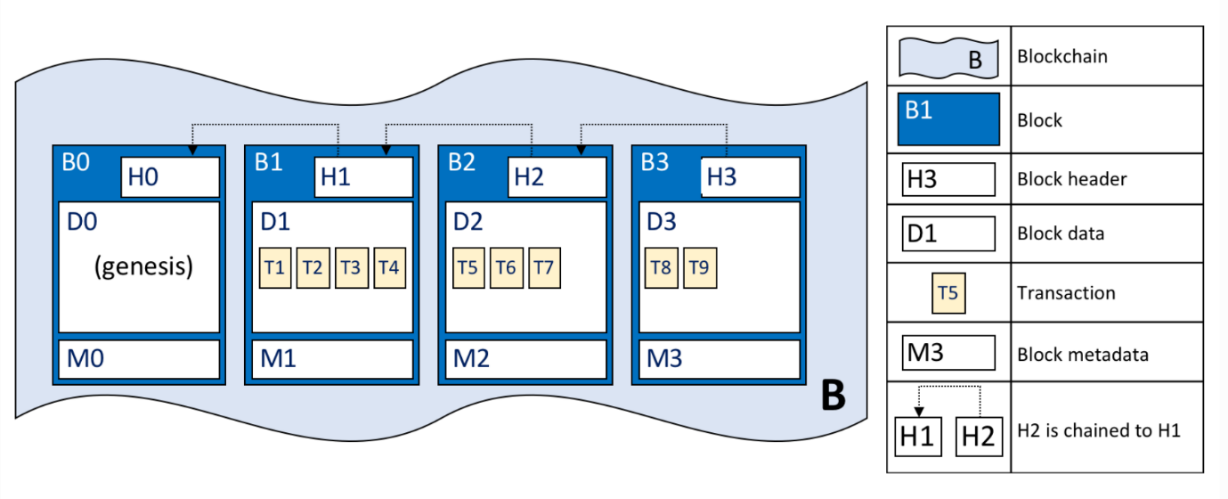
\includegraphics[width=13cm,center]{Figures/BlockchainStructure.png}
    \caption{The data structure underlying blockchain \cite{ADocumentation}. The first block is called the Genesis Block.}
    \label{Figure:BasicBlockchain}
\end{figure}

Blockchain removes the need for an intermediary, such as a bank, to mediate a transaction between 2 parties. External authorities are not required to validate the authenticity and integrity of data. It is a decentralised data structure that serves as the single source of truth to all nodes on the network creating trust between anonymous actors.



% -_____________________________________________________________________________

\subsection{Consensus Protocols}

The consensus protocol chosen determines how nodes validate and agree on any new transactions being added to the public ledger, and it varies between different blockchains. It makes sure that all nodes in a network have a consistent view of the ledger. This mechanism plays a crucial role in safeguarding against a variety of attacks that malicious nodes could attempt.
% -_____________________________________________________________________________

\subsubsection{Proof-Of-Work}

PoW is the consensus algorithm that couples voting weight with computing 
power. Thus it relies on computational resources to defend against the Sybil attack \cite{Sedlmeir2020TheMyth}.

\textbf{Miners} are nodes actively participating in the consensus-forming process. Miners compete 
to solve a computationally challenging mathematical puzzle in order to verify a group of transactions included in a block. In a brute-force manner, miners try to guess the right 'nonce' (number only used once) that when it is combined with the rest of the block header information and hashed, the hash has to have a certain number of leading zeros at the beginning. It is like trying to guess the number of a winning lottery ticket. It is challenging to produce (in terms of time and compute power) but easy to verify for other nodes \cite{Centieiro2021BitcoinCoding}. Once a node guesses the correct 'nonce', it broadcasts it to the rest of the network for validation. When most other miners have agreed on its legitimacy, the new block can permanently be added to the blockchain ledger, and the block proposer is rewarded with mining fees.

% -_____________________________________________________________________________

\subsubsection{Proof-Of-Stake}

PoS is a consensus protocol that relies on economic power rather than computational power to secure the network. It requires nodes called ‘validators’ to put up a set amount of their cryptocurrency at stake (as collateral). In exchange, they increase their chance of being randomly selected as the block proposer for the next round of transactions and consequently earn the block rewards that come with it \cite{King2012PPCoin:Proof-of-Stake}. In some implementations of PoW, the more a validator puts at stake, the higher their chance of being picked as the block proposer. If a validator submits a fraudulent transaction or tampers with transaction information, they risk losing their staked cryptocurrency and any block rewards they may have received, as other observing nodes always verify each new block \cite{Napoletano2022WhatAdvisor}. 

PoS is a much less energy-intensive design compared to PoW.

% -_____________________________________________________________________________

% -_____________________________________________________________________________

\section{Ethereum Basics}

Ethereum was introduced in 2015 by Vitalik Buterin as a blockchain platform with capabilities beyond cryptocurrency. It features smart contracts, which are segments of code that contain specific conditions. These contracts enable the creation of self-executing programs that activate automatically when the specified criteria are met. Ethereum's blockchain forms the backbone for a variety of applications, including Decentralized Applications (DApps), thanks to the functionality of smart contracts.

Nodes that communicate over a network following the 'ETH' protocol form the Ethereum network, also called the Ethereum 'mainnet'. These nodes contribute to maintaining and securing a globally agreed state of the Ethereum Virtual Machine (EVM). This was also described as 'one computer for the entire planet" by Ethereum co-founder Gavin Wood in 2016\cite{Ethereum:Industries}. 

The security of this network comes from a majority of nodes agreeing on the new change to the state of this EVM. In other words, agreeing on the next block to be permanently added to the blockchain ledger. Such nodes are paid in Ethereum's native cryptocurrency, \textbf{Ether (ETH)}, to run validator software that validates new blocks received over the peer-to-peer network.

Ethereum is a public, permissionless network, which means that anyone can access and participate in its operations. The interaction between a client and the Ethereum blockchain is enabled by the JSON RPC(Remote Procedure Call) API. When any user wants to complete a transaction with another user across the network, they:
\begin{enumerate}
    \item Need to specify the transaction amount
    \item Secure the transaction with their own private key
    \item Specify the tip they are willing to pay on top of the base transaction fees (both in 'gas' units) to incentivise a validator to validate and include their transaction in an upcoming block
\end{enumerate}

The ETH Execution client verifies the transaction request by checking things like whether the user has enough ETH to complete the transaction and if they have used the correct private key etc. \cite{EthereumEthereum.org}. 
This transaction request is then broadcasted to every other validator node over the execution layer 'gossip network'. Every validator adds this transaction to their local \textbf{'mempool'}. This is a collection of unverified transactions that are waiting to be processed and added to a new block.

During the pre-merge Proof-of-Work (PoW) era of Ethereum, \textbf{miners} competed to solve a mathematical problem using their computational power, and the first one to solve it was rewarded with Ether and earned the right to add a block to the blockchain. The difficulty of the problem automatically increased with the number of miners, making it computationally expensive and energy-intensive. 
% -_____________________________________________________________________________

% ________________________________________________________________________________-

% -_____________________________________________________________________________
\section{Post-Merge PoS Ethereum}

"The Merge", also known as the "Paris Upgrade", happened on 15$\mathrm{^{th}}$ September 2022. The Ethereum Blockchain switched from the older Proof of Work (PoW) to the Proof-of-Stake (PoS) consensus protocol. It was coined 'the Merge' as the Beacon Chain (a test network) was merged with the original Ethereum network. Both networks now operate simultaneously in layers. The older Ethereum chain is now known as the 'execution' layer (EL), now secured by the PoS 'consensus' layer (CL), formerly known as the Beacon Chain. 

The merge of the original chain with the Beacon Chain makes miners redundant. \textbf{Validator nodes} now secure the Ethereum network. 

\subsubsection{Full Nodes}
There is a popular mantra in blockchain, "Don't trust, verify" \cite{EthereumEthereum.org}. Following this altruistic mantra, running a Full Node allows a user to interact with the Ethereum Network in a trustless and self-sufficient manner. Everything can be checked and verified by your own node, removing the need to trust information from any other nodes in the network. 

Full Nodes need to run both an EL and CL client and must have  synchronised with the latest version of the blockchain in order to interact with the blockchain. 

\subsubsection{Validator Clients}
\label{ValidatorsLitRev}
To participate in the validation of transactions, Full Nodes must run an additional validator client and put 32 ETH at stake (currently equivalent to £45000) as collateral. Validator nodes are responsible for storing data, processing transactions and adding new blocks to the Ethereum blockchain permanently. Each Full Node can run multiple validator client instances, only limited by their computation and financial capacity.

Blocks are 'forged' by validators at a fixed tempo in PoS Ethereum. Every 12-second time \textbf{'slot'}, a pseudo-randomly selected validator gets to forge a new block and broadcast it to the rest of the network. Validators can choose which transactions in their mempool they will include in their next block. Validator client software executes these transactions locally, proposing a state change (such as a change in account balances). Once it completes enough transactions to fill up a block (there is a gas limit per block), it proposes this signed 'beacon' block to all other validators over the consensus layer (CL) network. This block is also wrapped in other information such as rewards, slashings, and attestations, which are discussed later.

32 time slots make up an \textbf{epoch}, usually around 6 minutes. For every slot, apart from selecting a block proposer (validator), a small committee of nodes is also randomly selected, whose votes determine whether the proposed block is valid or not. When these nodes receive the proposed block from the chosen validator, they pass it on to their Execution Layer Client (EL), where the block's data is verified. This includes ensuring the block corresponds to the correct slot, correct parent etc. Most importantly, the transactions in the block are re-executed to check that the proposed state changes are valid \cite{EthereumEthereum.org}. If the new block passes all checks, the nodes add it to their own local canonical blockchain. The one they believe to be the single source of truth. 

The algorithm judges each validator's actions and dishes out rewards and penalties at the end of each epoch accordingly. 

% \textbf{Sharding} \label{Sharding}
% One solution to increasing the number of transactions throughput on the network is sharding. It refers to splitting the entire Ethereum network into 64 portions called \textbf{shards} \cite{Buterin2020Annotated-spec/beacon-chain.mdEthereum/annotated-spec}. Each shard would contain its own independent state. It is an attempt at breaking up the blockchain into smaller parts no nodes are not responsible for processing or re-executing every single transaction broadcasted on the Ethereum network. Each shard is still connected to the main Ethereum chain cryptographically through merkle trees. \cite{EthereumEthereum.org} 


\textbf{Attestations}
\label{attestationLitRev}
Validators in a voting committee are expected to create, sign and broadcast their attestations(votes) to the rest of the network over the gossip network. These votes are either for or against the block being proposed in a specific slot. For each of the 64 committees formed, chosen aggregator nodes are responsible for aggregating their votes and propagating this information to the rest of the consensus nodes. If enough nodes agree on the block, it is added to the blockchain. 
\begin{figure}[h]
    \centering
    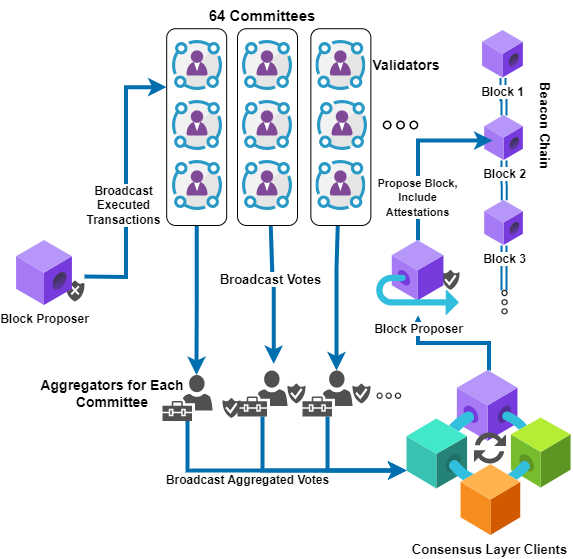
\includegraphics[width=13cm,center]{Figures/AttestationsDiragram.png}
    \caption{A diagram visualising the new block proposal and attestation process in PoS Ethereum}
    \label{Figure:AttestationsDiragram}
\end{figure}
 
\textbf{Staking ETH}

There are many different ways to stake ETH as a validator, as not everyone has access to or is prepared to lock up 32 ETH for an indefinite period. To get past this high barrier of entry, users can opt for solo staking, staking-as-a-service, pooled staking or centralised exchanges using 3$\mathrm{^{rd}}$ parties. 

The rewards of running a validator node come with some risks including:
 % ***shorten this section, kee relevant bits
 
\textbf{Slashing :}
This is when the algorithm destroys a portion of a validator's stake for behaving maliciously/ against the best interests of the network.

\textbf{Offline Penalty :}
If a validator goes offline for a number of days, they incur losses roughly equivalent to what they would have gained had they remained online. 

'The Merge' switched Ethereum's security model from computational power to \textbf{economic power}, which are comparable in many ways. Malicious attackers now need 51\% of the economic power of the entire Ethereum network instead of 51\% of the mining power for a successful attack. These severe economic punishments help to keep the network more secure than before while massively reducing the energy consumption of the network. 


% ----------------------------------------------------------------------

\subsubsection{Node Types}

Validator nodes are responsible for one of the two:
\begin{enumerate}
    \item Propose a new block by executing pending transactions from the mempool when randomly chosen as a block proposer for a slot
    \item Check blocks other validator nodes are proposing and attest to them by checking their validity and voting 
\end{enumerate}
As explained before, these nodes must stake 32 ETH in order to participate in securing the Ethereum network and earn rewards for adding blocks to the blockchain.

The version of the ledger stored by Full Nodes and validators is periodically pruned so that they don't hold the entire chain dating back to the Genesis block. \textbf{Archive Nodes} are a type of node that maintain an exact and complete copy of the entire blockchain dating back to the Genesis block. 

Apart from users looking to earn ETH or altruistic users wanting to secure the Ethereum network, not many users have the incentive to invest the time and resources to run a Full Node. This is why most users end up using centralised 3rd party hosted nodes. Client wallets like MetaMask and MyEtherWallet connect to a remote node in a non-cryptographically proven matter. New lighter node types, such as Light Nodes, were introduced to help make Ethereum accessible to more users, which in turn also makes the network more secure.

% \textbf{Light Nodes :}
% These are nodes that don't stake Ethereum. Instead, they are just used for accessing the network along with storing and processing the validation of the blocks within the network. These rely on full nodes as intermediaries to receive up-to-date information about the state of the blockchain. In essence, they are spectator nodes that constantly monitor the network and are witnesses that all activity complies with the rules.

% Because they are up-to-date nodes, they are allowed to interact with the Ethereum blockchain.  All they require is a simple installation of an ETH 2.0 node and a connection to the internet. This means the minimum requirements for the hardware required to run a light node is minimal and can be run on mobile devices.

% By design, they don't need to store or process the same amount of information that full nodes do. PoW light nodes only used download the headers of each block and were able to trace back. PoS light nodes also has to keep track of validators and their balances to stay on the chain with the most stake. This small amount of information allows light nodes to operate in a trust-minimised manner.


\subsubsection{Client Types and Synchronisation}

In the context of a blockchain, client software is software that connects users to each other in a peer-to-peer manner. Due to this cross-communication, these clients form a network where each client acts as a node. 

\textbf{Execution Layer Clients}

EL clients come in the form of community-maintained open-source software, formerly known as 'Eth 1' clients. Having a diverse share of client software being run on nodes participating in the network makes it more decentralised and reduces single points of failure.

Some popular EL clients include Geth, Nethermind, Besu and Erigon, written in languages such as Java, Go, and C\# \cite{EthereumEthereum.org}. 

\textbf{Consensus Layer Clients }

Following 'The Merge', CL clients, also known as 'Eth 2' clients, provide the security layer to the Ethereum network. This layer is responsible for the PoS consensus mechanism.

Some popular CL clients include Prysm, Lighthouse, Teku, Nimbus and Lodestar, written in languages such as Rust, Nim, Typescript and Go \cite{EthereumEthereum.org}. 

The latest network shares of each of these EL and CL clients can be found in \tref{Table:ClientShares} in \sref{Modelling}.

\textbf{Synchronisation} 
\label{SyncLitRev}

Synchronisation refers to a new node catching up to the latest version of the Ethereum Blockchain by retrieving the most up-to-date information. This is done by requesting data from peers. This data is cryptographically verified and used to build a local copy of the blockchain, treated as the single source of truth.

PoS Ethereum relies on the Consensus Layer for handling consensus logic and block propagation. Thus, synchronisation is a shared process between the EL and CL client. In order for the EL client to start verifying and syncing a local copy of the blockchain, the CL client has to download the block header. Only when the CL client provides the EL client with a header to use as a synching target can it cryptographically verify the chain of blocks being synced is valid. After this chain of block headers has been formed and validated, the rest of the blocks' information is downloaded \cite{2022DeveloperGo-ethereum}. This is the step that often takes the longest.

Many syncing modes exist, including Full, Snap, Fast and Light Sync.

\textbf{Full Sync }independently verifies the block provenance by re-executing the transactions starting at the Genesis Block. However, only the latest 128 blocks are actually stored in the Full Node, along with a few checkpoints representing older blocks. 

\textbf{Snap Sync }was developed by Geth developers (the prevailing EL client). It works similarly to a Full Sync, except it starts at a much more recent checkpoint to start its verification up to the front of the chain \cite{2022DeveloperGo-ethereum}.

Synchronisation time varies depending on the client software chosen as well the node's hardware configuration. It is not uncommon for syncing times to range between 12 hours and 6 days (see Appendix B).
% -_____________________________________________________________________________

% __________________________________________________________________________________________-
% -_____________________________________________________________________________

% __________________________________________________________________________________________-

\section{Carbon Emissions of Blockchain Technology }

Bitcoin, the world's largest cryptocurrency, currently holds a market cap of \$588 billion, with Ethereum trailing behind narrowly (\$242 billion market cap) \cite{BitcoinCoinMarketCap}. Most of these cryptocurrencies rely on the Proof of Work consensus, which by design uses energy-intensive processes to secure the network. Hence, it should not be surprising that they have huge adversarial effects on the environment. Empirical findings using the ARDL model show that increasing the volume of trading all cryptocurrencies results in higher energy consumption, with long-term effects on the environment \cite{Schinckus2020Crypto-currenciesConsumption}. \newline 

While the benefits of using decentralised transactional systems are appealing to many, it has become synonymous with inefficiency and disproportionate energy consumption \cite{DeVriesBitcoinsProblem}. Digiconomist's index suggests that if Bitcoin's energy was to be compared to that of entire countries, it would rank 38th in the world, finishing ahead of large countries like Chile and Bangladesh \cite{BitcoinDigiconomist}. The energy cost of redundancy due to decentralisation has become hugely problematic, inhibiting the wider adoption of cryptocurrencies. To put this into context, a comparison is often drawn between cryptocurrencies and traditional transactional systems such as Visa and MasterCard, which will always be more efficient due to their centralised nature \cite{Kohli2023AnSolutions}.  

\begin{figure}[h]
    \centering
    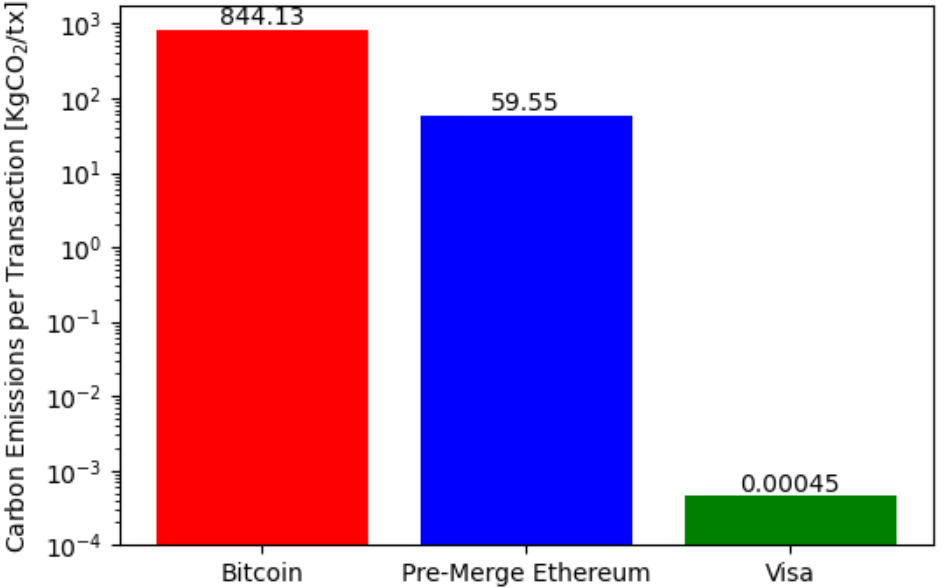
\includegraphics[width=13cm,center]{Figures/CarbonEmissionsPlot.png}
    \caption{Carbon emissions per transaction for Bitcoin, Ethereum 1.0 and Visa plotted on a logarithmic scale. Code is in Appendix C. Source: \cite{Kohli2023AnSolutions} }
    \label{Figure:CarbonEmissionsPlot}
\end{figure}

The stark difference in emissions per transaction is highlighted in \fref{Figure:CarbonEmissionsPlot}, especially due to using a logarithmic scale. These carbon emissions can be used as a proxy of environmental damage \cite{2022VisaReport}. This environmental damage linked to energy consumption renders it highly unsustainable.

Apart from cryptocurrencies, blockchain technology is increasingly being employed to track provenance in supply chains, especially drug-supply chains \cite{Labaran2021TheNigeria}. The literature contains numerous examples of such implementations using blockchain found in \tref{Table:DrugSupplyImplementations}, with some claiming to be low-energy solutions employing off-chain storage and non-PoW consensus mechanisms.

\begin{table}[!htb]
\centering
\begin{tabular}{|l"l|l|l|l|l|}
\hline
\textbf{Topic} &
  \textbf{\begin{tabular}[c]{@{}l@{}}Vaccine \\ Delivery \\ Solution\end{tabular}} &
  \textbf{\begin{tabular}[c]{@{}l@{}}Medication \\ Anti-fraud \&\\ Traceability\end{tabular}} &
  \textbf{\begin{tabular}[c]{@{}l@{}}‘Everyware’\\ Platform\end{tabular}} &
  \textbf{\begin{tabular}[c]{@{}l@{}}Analysis of \\ Blockchain in \\ Healthcare\end{tabular}} &
  \textbf{\begin{tabular}[c]{@{}l@{}}Drug \\ Traceability\\ Solution\end{tabular}} \\ \thickhline
\textbf{\begin{tabular}[c]{@{}l@{}}Blockchain \\ Platform\end{tabular}} &
  Ethereum &
  Ethereum &
  Hedera &
  \begin{tabular}[c]{@{}l@{}}Hyperledger\\ Fabric\end{tabular} &
  Ethereum \\ \hline
\textbf{\begin{tabular}[c]{@{}l@{}}Consensus \\ Algorithm\end{tabular}} &
  PoW &
  \begin{tabular}[c]{@{}l@{}}practical\\ Byzantine\\ fault tolerance\end{tabular} &
  \begin{tabular}[c]{@{}l@{}}Hashgraph\\ Consensus\end{tabular} &
  \begin{tabular}[c]{@{}l@{}}Redundant\\ Byzantine \\ fault tolerance\end{tabular} &
  PoW \\ \hline
\textbf{\begin{tabular}[c]{@{}l@{}}Type of \\ Operations\end{tabular}} &
  \begin{tabular}[c]{@{}l@{}}Public   \\ Permissioned\end{tabular} &
  \begin{tabular}[c]{@{}l@{}}Public   \\ Permissioned\end{tabular} &
  \begin{tabular}[c]{@{}l@{}}Public \\ Permissioned\end{tabular} &
  \begin{tabular}[c]{@{}l@{}}Private   \\ Permissioned\end{tabular} &
  \begin{tabular}[c]{@{}l@{}}Public\\ Permissioned\end{tabular} \\ \hline
\textbf{Currency} &
  Ether &
  None &
  None &
  None &
  Ether \\ \hline
\textbf{\begin{tabular}[c]{@{}l@{}}Off-chain \\ storage\end{tabular}} &
  Yes &
  None &
  Yes &
  None &
  Yes \\ \hline
\textbf{\begin{tabular}[c]{@{}l@{}}Customisable \\ Component\end{tabular}} &
  \begin{tabular}[c]{@{}l@{}}Ethereum\\ Smart \\ Contracts\end{tabular} &
  \begin{tabular}[c]{@{}l@{}}Ethereum\\ Smart\\ Contracts\end{tabular} &
  Yes &
  \begin{tabular}[c]{@{}l@{}}Docker\\ Container\end{tabular} &
  \begin{tabular}[c]{@{}l@{}}Ethereum\\ Smart \\ Contracts\end{tabular} \\ \hline
\textbf{\begin{tabular}[c]{@{}l@{}}Energy \\ Consumption\end{tabular}} &
  High &
  Low &
  Very Low &
  Low &
  High \\ \hline
\textbf{Source} &
  \cite{Musamih2021Blockchain-BasedVaccines} &
  \cite{Zhu2020ATraceability} &
  \cite{Platform}, \cite{TechnologyLtd} &
  \cite{Mettler2016BlockchainHere} &
  \cite{Musamih2021AChain} \\ \hline
\end{tabular}
\caption{Several implementations of drug-supply chain solutions that use blockchain technology, with 3 implementations using Ethereum 1.0}
\label{Table:DrugSupplyImplementations}
\end{table}

However, newly established independent blockchains, whether intended for cryptocurrency or provenance purposes, often struggle to maintain the two primary benefits of blockchain technology, either through security breaches due to a lack of users or centralization through permissioned blockchain solutions. 51\% attacks occur when a malicious miner or group controls over 50\% of a network's computational power. Small blockchains with few participants are more vulnerable as it is easier for a malicious actor to acquire the necessary computational power, leaving the blockchain susceptible to tampering and theft \cite{Redman2021PrivacyErased}.









% _______________________________________________________________
% -_____________________________________________________________________________

% __________________________________________________________________________________________-
% -_____________________________________________________________________________

\subsection{Mathematical Modelling}
\label{MathematicalModellingLitRev}

Modelling is about making some assumptions in order to simplify a complex system and test a hypothesis. There are a number of approaches for scientific model building, descriptive and rule-based modelling \cite{SayamaINTRODUCTIONSYSTEMS}. This paper employs the latter.

\textbf{Rule-based modelling} involves coming up with certain dynamic rules and limitations that can explain the behaviour of a system. It is all about capturing how the model will behave over time, usually done using quantitative methods.

Observations must be turned into mathematical equations, but this can be challenging as the system's unique properties may be ones we are not familiar with (for example, large networks and nonlinearity). A book on modelling complex systems claims the 4 things to keep in mind when modelling include \cite{SayamaINTRODUCTIONSYSTEMS}:

\begin{itemize}
    \item The key research questions that need to be addressed
    \item To answer the research questions, what scale is most appropriate to describe the systems, microscopic or macroscopic
    \item How the system is structured
    \item What are all the possible states of the system, and how it changes over time
\end{itemize}

This study uses the microscopic details of the Ethereum protocol (how attestations are handled) to model its macroscopic effects at scale (increase in overall energy usage). 



% ____________________________________________________________________---

% ______________________________________________________________________________
% -_____________________________________________________________________________

% __________________________________________________________________________________________-


\section{Modelling PoW Energy Consumption}

This section aims to analyse a wide range of papers on the topic of energy consumption of blockchain. The steps for a structured literature review laid out by \cite{Crosby2015BlockChainBitcoin} are loosely followed. 

Most papers in this niche field of research emphasise Bitcoin and PoW cryptocurrencies. It shows a clear gap in the literature for more work to be done on modelling the electricity consumption of non-PoW blockchains, as this study intends to do.
% -_____________________________________________________________________________

Paper \cite{Sedlmeir2020TheMyth} attributes almost all the energy consumed by PoW blockchains to the PoW consensus mechanism alone. The other factors contribute a negligible amount of energy in comparison. However, estimating the energy consumption of blockchain consensus mechanisms can be challenging due to the scarcity of accurate information on the number of network participants and their hardware configurations. The same study also confirms that Proof-of-Work (PoW) blockchains consume a disproportionate amount of energy relative to the actual utility they offer. When comparing PoW electricity estimates to those of non-PoW blockchains, the results were several orders of magnitude lower for non-PoW blockchains \cite{Sedlmeir2020TheMyth}. Due to non-PoW consensus algorithms having such a small energy footprint, their energy consumption cannot solely be attributed to its consensus algorithm but rather to a range of other factors too, which come with having a large decentralised network. This is discussed further in \sref{LitRevExistingModels}. 

\begin{figure}[h]
    \centering
    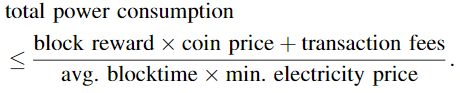
\includegraphics[width=8cm,center]{Figures/SimplePoWModel.png}
    \caption{A simple model estimating the upper bound of electricity consumption of a PoW blockchain. Source: \cite{Sedlmeir2020TheMyth} }
    \label{Figure:SimplePoWModel}
\end{figure}

Energy consumption in many PoW-focused papers is attributed to metrics like block rewards, coin price, transaction fee, average block time and hashing difficulty which are all publicly available and reliable metrics, \cite{Mcdonald2022EthereumEstimate}. Such a model is shown in \fref{Figure:SimplePoWModel}.

% -_____________________________________________________________________________
Another data-driven study collected and analysed publicly available data to derive a joule per hash (per 'nonce' value calculated) value based on a small number of direct measurements from a small testbed network \cite{Cole2018ModelingAlgorithms}. Using a LASSO (Least Absolute Shrinkage and Selection Operator) regression model, the researchers were able to estimate the energy usage of PoW cryptocurrencies with 92\% accuracy. The same cannot be done for PoS blockchains due to the lack of data availability and the vast range of factors affecting its energy consumption outside of the consensus protocol itself.

Digiconomist \cite{BitcoinDigiconomist} and CBECI \cite{CambridgeCBECI} are two well-known real-time models used to estimate the energy consumption of Bitcoin. These are highly credible models and have been referenced many times in the wider literature, such as \cite{Cole2018ModelingAlgorithms}, \cite{Lei2021BestRecommendations}, and \cite{Erdogan2022AnalyzingSustainability}, \cite{Platt2022TheProof-of-Work}, respectively. Both models use live tracking of Bitcoin's price and mining hash rate to maintain accuracy but take different approaches to arrive at similar estimates. Digiconomist's top-down approach estimates the total revenue earned by USA-based Bitcoin miners. It assumes that 60\% of this revenue is spent on operational costs, primarily electricity, in the case of PoW. By using the global average electricity costs, the model is able to calculate Bitcoin's energy consumption. In contrast, CBECI uses a bottom-up approach, focusing on selecting contemporary mining equipment that maximises the number of hashes computed per Joule of energy used. The model then uses a profitability threshold to extrapolate Bitcoin's annual electricity consumption. This paper takes inspiration from both approaches introduced by these models to develop a model for non-PoW blockchains.





% __________________________________________________________________________________________-
% __________________________________________________________________________________________-


\subsection{ Electricity Consumption of PoS Blockchains }
\label{LitRevExistingModels}

There is a large gap in the literature on this niche field of research. This section analyses the work done in this area and why it needs to be improved upon.

A study by Powell et al., aimed at making recommendations for building greener blockchains, suggested a simple formula to calculate the energy of the Polkadot blockchain that employs PoS consensus \cite{Powell2021AWARENESSBLOCKCHAIN}. Their model was the first of its kind, and it follows: 
\begin{align}
   \boldsymbol{\mathrm{\text{Polkadot Energy Consumption } = }}
   &\boldsymbol{\mathrm{\text{ Energy per server }* \text{ number of servers } } } \nonumber\\
   &\boldsymbol{\mathrm{* \text{ 24 hours } *\text{ 365 days }}} \nonumber
\end{align}

A recent study by UCL Centre for Blockchain Technologies \cite{PlattDiscussionProof-of-Work} built upon this equation by establishing a mathematical relationship between validator number, network load and hardware configuration to estimate the energy consumption of the PoS consensus protocol in isolation. Their approach was to build upon past literature using new data sets from various sources, including empirical data from CCRI report \cite{CryptoCarbonRatingsInstitute2022TheNetwork} and other publicly available metrics while avoiding time-consuming first-hand experimentation, just like this study aims to do. 

\begin{align}
   \boldsymbol{\mathrm{\text{Energy Per Transaction} = }}
   &\boldsymbol{\mathrm{\frac{\text{ Energy per Validator }* \text{ Number of Validators } }{\text{ Number of Transactions }}} } \nonumber\\ \nonumber
\end{align}

Their generalised model performs well for a few different PoS blockchains, with Ethereum being one of them. In fact, R3, a private company that run the Corda blockchain have also used the same equation to estimate its energy consumption \cite{JustBlog}. However, amidst this generalisation, the UCL study makes a critical mistake of not differentiating between validators (currently $\sim$500,000 \cite{EthereumEthereum.orgc}) and Full Nodes ($\sim$15,000 \cite{NodewatchAnalytics}). Their model only considers validators and estimates only the PoS consensus protocol’s energy usage in isolation. Thus, incomplete in its calculation of network-wide energy consumption by ignoring factors such as the 'Full Nodes' that aren't actively participating in forming consensus but greatly contribute to securing the blockchain. Such factors have not been ignored in the model proposed by this study. The UCL study also relies on speculative assumptions as it was written before Ethereum’s upgrade to PoS consensus (now the world’s largest PoS blockchain). Hence, the most significant PoS blockchain was not included in its study.

The future work mentioned in the study is closely aligned with the focus of this study, which aims to build a more comprehensive model by incorporating additional factors and considering different node types.


\textbf{The CCRI Study } 
\label{CCRIModelLitRev}
The state-of-the-art research conducted by Crypto Carbon Ratings Institute focuses specifically on the energy consumption of post-merge PoS Ethereum. It provided the most up-to-date empirical data that has been cited in other studies such as this one \cite{CryptoCarbonRatingsInstitute2022TheNetwork}. These researchers decided on 6 commodity hardware configurations that they ran idly for base power consumption figures and then ran each major EL and CL client software separately, taking 48-hour electricity measurements. The data was used in their equation (detailed in \sref{CCRIBaseEqnSection}), which was formulated using a combination of experimentation and prior domain knowledge. The accuracy of the model was confirmed by comparing the actual measurements from running Full Nodes to their estimated values, which were found to be highly precise.

Assumptions and shortcomings of this study:
\begin{enumerate}
    \item Different combinations of clients were run to form Full Nodes. However, the next step of running a validator client on the Full Node was not taken due to the barrier of staking 32 ETH. The effects of running a validator client on top of a Full Node were assumed to be negligible.
    
    \item The synchronisation energy consumed whilst bootstrapping Full Nodes was not considered.
    
    \item Other node types, such as Light and Archive Nodes, were not considered, presumably due to assuming that they would have negligible effects.

    \item The electricity data was collected using computer software, but there is no information available on the type of power supply and mainboard used in the experiments. Therefore, the measurements only account for the electricity consumed by the computer itself and do not factor in the power draw 'At-Wall' or any electrical inefficiencies. \cite{Warkozek2012ACenters}
\end{enumerate}
 


% -_____________________________________________________________________________


% Quick intro on AVX operations, what is TDP and why that is the upper limit of CPU power consumption
% AVX instructions enable the processor to perform multiple floating-point operations at the same time, resulting in faster computation and improved performance. \cite{Schuchart2016TheScale}

% ______________________________________________________________________________
% -_____________________________________________________________________________

% __________________________________________________________________________________________-

% \section{Key Points Covered}

\setcounter{chapter}{3}
\chapter {Methodology}

\section{Model Development Steps}
\begin{enumerate}
    \item Conduct a comprehensive analysis of existing models for PoW and PoS blockchains. Select a state-of-the-art model that employs a bottom-up approach, making it easier to incorporate new factors into it \cite{CambridgeCBECI}. Provide a comprehensive explanation of its components.

    \item Acquire a deep understanding of the interplay of microscopic factors and their macroscopic effects in Ethereum PoS \cite{MarionAnModelling}. With this knowledge, consider the limited 'post-merge' data available and identify 2-3 factors that can be integrated into the base model.

    \item Analyse data and literature relating these factors to electricity consumption in various contexts. Adhering to the principles of Rule-Based Mathematical Modelling outlined in \sref{MathematicalModellingLitRev}, develop equations related to PoS Ethereum, either by adapting existing equations to the given context or through modelling observed behaviours.

    \item Incorporate these equations into the base model. Estimate the network shares of users employing different hardware, client, and node configurations, and assign weights to different parts of the equation where possible \cite{CCRI:Institute}.

    \item Determine the contemporary metrics (e.g., gas fees, transaction count, etc.) required to implement the model proposed along with competing models. Implement all models using the same metrics to produce easily comparable values (like energy consumption per transaction) to facilitate the evaluation of the model's results \cite{CryptoCarbonRatingsInstitute2022TheNetwork}.

\end{enumerate}

\section {Evaluation Metrics}

\subsection{Quantitative}
\label{MethoologyErrorQuant}
The aim of a validation metric is to be able to assess the predictive capability of a mathematical model \cite{Kat2012ValidationError}. Results for comparison will be obtained by implementing other similar mathematical models found in the literature. Most relative-error measures compare true observed values to prediction results. However, since all models estimate the energy consumption of Ethereum, there is no true value. Thus, selecting an appropriate quantitative error measure is challenging. 

The magnitude error, which compares the relative orders of magnitude between two functions, could be used as a means of validating the results obtained. To calculate the magnitude error using \eref{eqn:ErrorMeasureEqn}, results from an experimental model with scientific data will be treated as the true value, $\boldsymbol{\mathrm{m}}$, while estimates from our 'Model-A' will replace prediction value, $\boldsymbol{\mathrm{p}}$ \cite{RussellErrorMeasure}. The suggested upper bound for a result being acceptable is $\boldsymbol{\epsilon_\mathrm{rme} \leq 0.2}$.

\begin{align}
\label{eqn:ErrorMeasureEqn}
    &\boldsymbol{\epsilon_\mathrm{rme} = \mathrm{sign(rme)} * \log_{10} (1 + |\mathrm{rme}|)}
    &\boldsymbol{ \mathrm{rme} = \mathrm{\frac{\mathrm{\sum\limits_{i=1}^{N} p_{i}^{2}} - \mathrm{\sum\limits_{i=1}^{N} m_{i}^{2}}}{\sqrt{\mathrm{\sum\limits_{i=1}^{N} p_{i}^{2}} * \mathrm{\sum\limits_{i=1}^{N} m_{i}^{2}}}}}}
\end{align}

% --------------------------------------------------------------------
\subsection{Qualitative}
\label{QualModelEvalMEthodology}
 It would be a near-impossible task to successfully verify the model through h simulate PoS Ethereum without losing its microscopic characteristics that this study relies on to improve upon the base model. Some qualitative techniques that can instead be used to verify the model include the following \cite{Al-Aomar2015ModelTechniques}:

\textbf{1. Thorough Examination of Model Inputs - } During development, the input values for each part of the model will be obtained only from scientific sources. If infeasible, anecdotal data from multiple sources must be averaged as a substitute. A 'valid' input is defined as being:
\begin{enumerate}
    \item Correct
    \item Relevant to the real-world system being modelled
    \item Being used in the model similar to the way they would be used by the real-world system being modelled
\end{enumerate}  

\textbf{2. Detailed Documentation of Model Logic - }
Every decision made during the formulation of the model must be clearly documented and well-justified using observed data or domain-specific knowledge. All assumptions will be highlighted using bold formatting.


\textbf{3. Thorough Examination of Model Outputs - }
The model's results must lie in a 'reasonable' range when compared to competing model's results \cite{Al-Aomar2015ModelTechniques}. Any discrepancies between Model-A and other models must be clearly addressed in the discussion section.   

\section {Data Gathering}

The primary scientific data source in this field is from the CCRI study \cite{CryptoCarbonRatingsInstitute2022TheNetwork}, which has been referenced in most other studies in this emerging area of research \cite{IbanezTheExpansion}. In addition to this data, a variety of sources, including blockchain crawlers for obtaining metrics such as transaction counts, and anecdotal or non-scientific sources like Reddit and Discord communities (where reputed users share their measurements), were collected and averaged. See Appendix A.

The CCRI \cite{Ccri-apiOverview} and Etherscan \cite{EtherscanProvider} APIs will be used to pursue a data-driven approach to modelling. The majority of indices publicly accessible on the CCRI website display annualized values for daily estimates. These values will be divided by 365 to acquire accurate daily figures.

% \section {Modelling The Energy Consumption Using Domain Knowledge}

% *Define everything in your modelling world, what your definition of everything is

% We care about the power coming from the grid. The AC 'At-Wall'. We gather estimations for the recommended configuration of hardware for Ethereum nodes running validator clients. 

% Also decide on which way of data gathering is better. Prepare a table of online users claiming their power consumption. Also, estimate the power consumption of the recommended configuration of hardware through manufacturer websites. This is then compared to the data from the \cite{CryptoCarbonRatingsInstitute2022TheNetwork} report actually running a single validator node to check if this bottom-up hardware estimation approach is valid. 

% Knowing the fact that increasing the number of validator clients on a single machine increases the power consumption logarithmically, we apply this assumption to the CCRI equation. We also need to account for power inefficiency of the computer by adding a factor to this equation. The report does not mention the power supply or mainboard used.

% Also need to add the syncing energy into the equation as it is not a short process. Need to model this, depending on the data and add it to the equation. (possibly for every combination of CL and EL client)
% ------------------------------------------------------------------

\section {Project Management}

Agile project management practices were employed during the course of this project. 

\subsection{Task Management}

Given the frequent topic changes throughout the project, adopting an agile methodology was critical to the success of this project. Todoist, a task management tool, was utilised for micro-task management. Its visual task board enables task categorisation by importance level, date, and macro-tasks, as demonstrated in Appendix E. Various self-set milestones were dated into my task list and, when complete, updated into my Gantt chart.

Macro-level task management was accomplished through implementing a Gantt chart. These tasks underwent drastic changes monthly due to the newfound knowledge of the research area and progress in the technical section. The latest Gantt chart is shown in \fref{Figure:ganttUpdated}, with the original version in Appendix G. 

\subsection{Time Management}

The Gantt chart also facilitated macro-level time management by allocating time for each major project task across both semesters. Realistic allocations were made and updated monthly, accounting for other coursework and unexpected delays. 

Furthermore, brief summaries of relevant literature papers read during the course of this project were recorded in a Word document (Appendix F). This approach allowed for the efficient organisation of ideas and prevented rereading papers, saving time. 


\begin{figure}[!htb]
    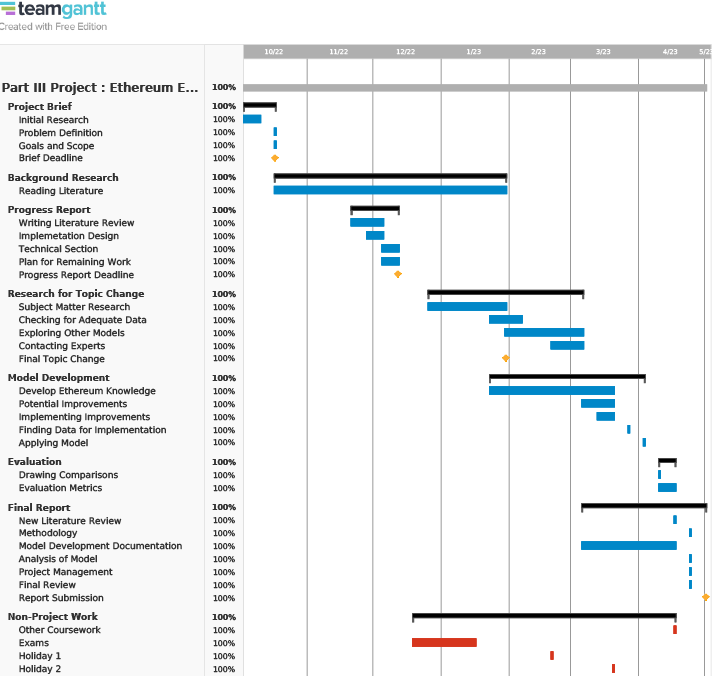
\includegraphics[width=14cm,center]{Figures/ganttUpdated.png}
    \caption{Latest version of the Gantt Chart. An older version of the Gantt Chart}
    \label{Figure:ganttUpdated}
\end{figure}



\subsection{Risk Management}

Forseen risks associated with taking on such a novel project have been compiled into \tref{Figure:RiskTable}, ordered by descending risk score, calculated as the quotient of $\mathrm{Probability * Impact}$.

\begin{table}[!htb]
    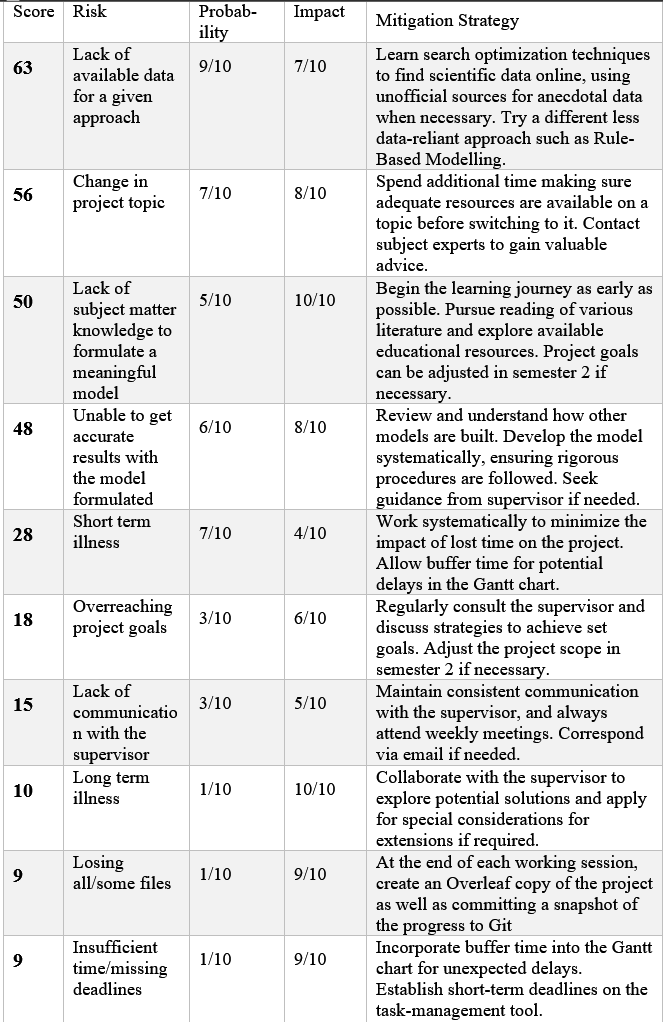
\includegraphics[width=14cm,center]{Figures/RiskTable2.png}
    \caption{Risk Analysis table taken from the progress report submission.}
    \label{Figure:RiskTable}
\end{table}
\setcounter{chapter}{4}
\chapter{Modelling The energy Usage Of Ethereum}
\label{Modelling}

% ____________________________________________________________________________
\section{Summary}

This chapter constitutes the technical section of this study, comprising of creating our mathematical model to estimate the energy consumption of PoS Ethereum, called 'Model-A', and then gathering data to implement that model amongst others for comparative analysis. 
% ____________________________________________________________________________

% %  Model-AAAAAAAAAAAAAAAAAAAAAAAAAAAAAAAAAAAAAAAAAA
% \subsection{Model-A}
% From the research,it seems like power usage is usually not the limiting factor but rather the storage space needed to run validators.

% The recommended hardware for a validator one is shown in table \_\_ of the appendix as well as in the table below. \_\_

% So according to this hardware recommendation, we could estimate the power usage depending on statistics provided by manufacturers. Let's assume the same configuration of hardware as in the \cite{CryptoCarbonRatingsInstitute2022TheNetwork} (They don't mention type of power supply and mainboard).  According to data from the manufacturers, the power consumption for this configuration comes out to the following: 

% \begin{itemize}
%     \item Processor TDP - 105W
    
%     \item An SSD uses 5W while Active
    
%     \item Every 8GB of memory uses 3W, so 16GB of memory will use 6W
    
%     \item For a solo validator set-up (non-specialised hardware), miscellaneous components are likely to use another 30W
    
%     \item As 92\% efficiency is common, the machine will likely peak at 178W of AC power drawn from the wall
    
%     \item The machine will run at idle power consumption 50-90\% of time, so on average it would use around 50-100W
    
% \end{itemize}

% _____________________________________________________________________________
%  Model-AAAAAAAAAAAAAAAAAAAAAAAAAAAAAAAAAAAA
\section{'Model-A': Parametric Modelling with Prior Domain Knowledge}

% \textbf{Light Nodes}
% Light nodes require much less computational power to run compared to a full node, yet, they still work in a trust-minimised way. This is due to their cryptographically proven way of using block headers of the blockchain to verify the information they are receiving from a full 
% node themselves. 

% Light clients send out a lot of requests, a lot more than full nodes. For example, they might need to check the balance of certain accounts to verify the information they are receiving cryptographically. This large number of simple requests ends up requiring more network bandwidth than full nodes \cite{WhatTechnologies}. We also know that light clients are designed to be run on minimal devices such as mobile and IoT devices. The amount of computational and storage resources required by a light node is orders of magnitude lower than a full node. It requires only about 100MB of storage \cite{WhatTechnologies}. This fact can be used to model this. These devices also sync with the latest blocks using checkpoints in seconds instead of hours like a full node.

% _____________________---stage 1
\subsection{The base model}

First, the base CCRI equation \cite{CryptoCarbonRatingsInstitute2022TheNetwork} upon which 'Model-A' will be built is introduced below. The symbols denoting each metric have been adapted to the context of this study.

\begin{center}
A Consensus Layer Client's power usage [in Wh]:
\begin{equation*}
    \boldsymbol{\mathrm{P}_{CL}}
\end{equation*}

An Execution Layer Client's power usage [in Wh]:
\begin{equation*}
    \boldsymbol{\mathrm{P}_{EL}}
\end{equation*}
 
 An Idle client's power usage [in Wh]:
 \begin{equation*}
    \boldsymbol{\mathrm{P}_{ID}}
\end{equation*} 

Mean energy usage for each of the 3 client types is denoted by: 
\begin{equation*}
  \boldsymbol{\mathrm{{\overline{P}}_{CL}}}\quad      \boldsymbol{\mathrm{{\overline{P}}_{EL}}}\quad  \boldsymbol{\mathrm{{\overline{P}}_{ID}}}   
\end{equation*}

The total number of consensus and execution layer client combinations that can be run:
\begin{equation*}
    \boldsymbol{n}
\end{equation*}

The known share [in \%] network running a specific combination of consensus and execution layer client:
\begin{equation*}
    \boldsymbol{\phi}_{EL,CL} 
\end{equation*}

The total share of the network occupied by all ${n}$ tested combinations of CL and EL clients is denoted by:
\begin{equation*}
    \boldsymbol{{\pi} = \displaystyle\sum\limits_{i=1}^{n}{\phi_{EL,CL}}}
\end{equation*}

The final CCRI equation for the weighted energy consumption of an average node for each combination of CL and EL client \cite{CryptoCarbonRatingsInstitute2022TheNetwork}: 
\label{CCRIBaseEqnSection}
\begin{equation}
\boldsymbol{\frac{\displaystyle\sum\limits_{i=1}^{n}{ \left({\left(\mathrm{\overline{P}}_{ID} + \mathrm{\overline{P}}_{CL} + \mathrm{\overline{P}}_{EL}\right)} * {\phi_{EL,CL}} \right)}}
 {\pi}}\label{eqn:CCRI}
\end{equation}
\end{center}

The CCRI model has been validated via experimentation as presented in its report, establishing it as a reliable foundational model \cite{CryptoCarbonRatingsInstitute2022TheNetwork}. 'Model-A', proposed in this study, enhances this base model by addressing shortcomings 1 and 2 mentioned in \sref{CCRIModelLitRev}.
% ____________________stage 1

\subsection{Improvement 1 : Adding the Synchronisation Energy} 

 \eref{eqn:CCRI} ignores the energy expended during the bootstrapping stage of setting up a node - the synchronisation process. 'Geth' is currently the most dominant ( see \tref{Table:ClientShares}) and long-standing Ethereum EL client. Its snap-sync mode is the most commonly used synchronisation method as it strikes a great balance between independent verification and sync speed (explained in \sref{SyncLitRev}).
% DIAGRAM FOR SNAP SYNC

 All synchronisation methods are very energy-intensive, and Geth snap-sync is no exception. It works by downloading and verifying the headers of blocks, in small chunks. Simultaneously, it begins downloading the state-trie for each of these blocks and cryptographically verifying this by re-calculating it locally. These computationally intensive processes utilise the node's CPU at its maximum capacity.

  % keeping Intel i5-1135G7 in mind
A simple model for calculating the energy consumption of a CPU is shown below \cite{PelleyUnderstandingPower} :

\begin{equation*}
    \boldsymbol{\mathrm{P}_{Total} = \mathrm{P}_{idle} + \left({\mathrm{P}_{max} - \mathrm{P}_{idle}}\right) * \mathrm{U}}
\end{equation*}

$\boldsymbol{\mathrm{P}_{Total}}$ is the total energy consumption of a CPU.\\
$\boldsymbol{\mathrm{P}_{idle}}$ and $\boldsymbol{\mathrm{P}_{max}}$ denote the power consumption of the CPU in an idle state and under maximum load, respectively.\\
$\boldsymbol{\mathrm{U}}$ varies between 0 and 1, with 1 representing the peak compute capacity of the CPU.

To capture only the energy consumption of the syncing process, we \textbf{assume} the CPU to be operating at its maximum capacity, hence taking $\boldsymbol{\mathrm{U}}$ to equal 100\%, or $\boldsymbol{1}$ for the sake of simplicity. This negates the need for $\boldsymbol{\mathrm{P}_{idle}}$ to be included in the equation, leaving:

\begin{equation*}
    \boldsymbol{\mathrm{P}_{Total} = {\mathrm{P}_{max}}}
\end{equation*}

Study \cite{Schuchart2016TheScale} shows that a CPU cannot continuously operate at its maximum capacity for computationally intense applications. To cope, it reduces its frequency, maintaining operations within its thermal power limitation, the TDP. Hence, the TDP can be used as an accurate substitute for the energy consumption of a CPU under high \textbf{sustained} load. The TDP (Thermal Design Power) for any CPU, $\boldsymbol{\mathrm{P}_{TDP}}$, can easily be found on the manufacturer's website.
\label{TDPReasoning}
\begin{equation*}
    \boldsymbol{\mathrm{P}_{max} = {\mathrm{P}_{TDP}}}
\end{equation*}

While the CPU is being utilised at maximum capacity, the node also begins storing this information locally to assemble a local copy of the chain. This storage process requires speeds that hard drives cannot keep up with. This fact is reinforced by the hardware specifications in \tref{Table:RecommendedHardware}, which specifically recommended using an NVMe SSD (Non-Volatile Memory Express Solid State Drive). These are much faster than traditional hard drives and expend more energy as a consequence. 

\begin{table}[h]
\centering
\begin{tabular}{|l|l|}
\hline
Full Node        & \begin{tabular}[c]{@{}l@{}}Quad Core Processor, \\ 2TB NVMe SSD , 16GB memory\end{tabular}                            \\ \hline
Archive Nodes               & \begin{tabular}[c]{@{}l@{}}Quad Core or Dual Core Hyperthreaded \\ Processor, 12TB NVMe SSD, 16GB memory\end{tabular} \\ \hline
Minimum for Full Nodes & \begin{tabular}[c]{@{}l@{}}Dual Core Hyperthreaded, \\ 1TB SSD, 4GB memory\end{tabular}                          \\ \hline
\end{tabular}
\caption{Hardware configurations for running various node types, recommeded by Geth developers \cite{2022DeveloperGo-ethereum}}
\label{Table:RecommendedHardware}
\end{table}

Thus, the energy usage of an NVMe SSD actively in use [in Wh] needs to be accounted for. This is denoted by:
\begin{equation*}
    \boldsymbol{\mathrm{P}_{SSD} } 
\end{equation*}

Often, it takes days to complete the synchronisation process. EL clients take most of the synchronisation time while the CL client contributes a tiny fraction \cite{Ethereum/go-ethereum:Protocol}. Hence, we \textbf{assume} the time it takes to complete the synchronisation process can be solely attributed to the EL client [in hours], denoted by:
\begin{equation*}
    \boldsymbol{\mathrm{T}_{EL}}
\end{equation*}

Combining the aforementioned factors results in the total power expended during the synchronisation process to be denoted as $\boldsymbol{\mathrm{P}_{SNC}}$ where:
\begin{equation}
    \boldsymbol{\mathrm{P}_{SNC} = \mathrm{T}_{EL} * \left({\mathrm{P}_{TDP}} + \mathrm{P}_{SSD}\right)} \label{eqn:Sync}
\end{equation}

 This bootstrapping process, respresented by \eref{eqn:Sync}, can be integrated into the base model (\eref{eqn:CCRI}) in the following way:

\begin{equation*}
    \boldsymbol{\mathrm{P}_{SNC} +  {\frac{\displaystyle\sum\limits_{i=1}^{n}{ \left({\left(\mathrm{\overline{P}}_{ID} + \mathrm{\overline{P}}_{CL} + \mathrm{\overline{P}}_{EL}\right)} * {\phi_{EL,CL}} \right)}}
 {\pi}} } 
\end{equation*}

Which simplifies to:

\begin{equation}
     \boldsymbol{\left({\mathrm{T}_{EL} * \left({\mathrm{P}_{TDP}} + \mathrm{P}_{SSD}\right)}\right) +  {\frac{\displaystyle\sum\limits_{i=1}^{n}{ \left({\left(\mathrm{\overline{P}}_{ID} + \mathrm{\overline{P}}_{CL} + \mathrm{\overline{P}}_{EL}\right)} * {\phi_{EL,CL}} \right)}}
{\pi}} } \label{eqn:CCRISync}
\end{equation}
\label{AdditonalNodesReasoning}
\newline \newline
% --------------------------------------------------------
\subsection{ Improvement 2 : Running additional validators on each node}


Contemporary data suggests that there are roughly 11-15000 nodes connected to the Ethereum network at any given moment \cite{NodewatchAnalytics}; meanwhile, there are 561,472 active validator clients \cite{EthereumEthereum.orgc}. As explained in \sref{ValidatorsLitRev}, it is known that most solo-stakers run 1-1000 validator instances per physical node. With more specialised hardware, 2500-7000 validators can be run on a single node \cite{Kaushal2022ValidatingConference}. 

Leveraging this knowledge, it can be deduced that adding each additional validator must have negligible effects on a given node. \fref{Figure:validatorIncrease} shows the effects on the CPU usage as the number of additional validators being run increases on a single Full Node, gradually.

Storage space was falsely expected to be a limiting factor to the increasing number of additional validators, as a single validator takes up almost 2TB of storage. However, after the first validator already has synchronised its local copy of the blockchain, adding more validators only requires storing a few extra cryptographic keys per validator.

\begin{figure}[htb!]
    \centering
    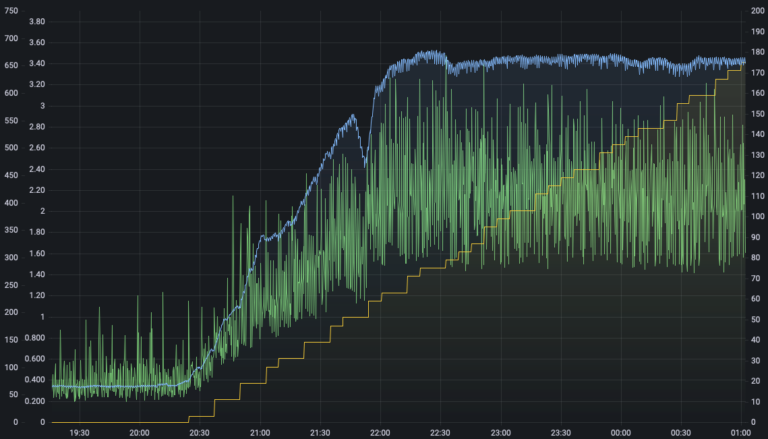
\includegraphics[width=15cm,center]{Figures/cpuValidatorsGossip.png}
    \caption{Graph from \cite{Sutton2022ExploringSymphonious} plots CPU usage (green line, scale up to 3.80 in GHz) and gossip network messages per second (blue line, scale up to 750 messages/sec ), against the number of additional validators being run increase (yellow line, scale up to 200 clients).}
    \label{Figure:validatorIncrease}
\end{figure}

As expected, a linear correlation can be seen between the increasing additional validators and the CPU usage, but only up to $\sim$65 validators. However, after the 60-70 validator range, the CPU usage and the gossip messages per second level off and seem unaffected by the steadily increasing validators. 

In each epoch (32 slots), 32 randomly selected block proposers propose one block per slot. The remaining validators are not only assigned to one of 64 voting committees of one of the 32 slots that they need to attest to (vote on a new block's validity). This is depicted in \fref{Figure:AttestationsDiragram} (\sref{AttestationsLitRev}). Each of these committees publish their attestations into separate gossip topics. Unaggregated votes from these committees are aggregated and pushed out on specific gossip channels by certain validators chosen to do so. 

Full Nodes that are not running validators will only subscribe to the gossip topics that push out aggregated votes. But with each new validator that is run, it subscribes to a new gossip channel associated with the committee it joins that has unaggregated votes. As there are 64 committees per slot, up to 63 additional validators, the node has to subscribe to and process more gossip messages. However, past this, there are no new gossip topics left to subscribe to, and the CPU usage and rate gossip messages per second levels off, as shown in \fref{Figure:validatorIncrease}.

To model this behaviour, logarithmic and exponential functions were explored. Through extended experimentation and application of prior mathematical knowledge, it was found that the exponential decay function (increasing form), \eref{eqn: ExpDecayGeneral}, most accurately matches the characteristics desired. Initially, it increases almost linearly at a slow rate before levelling off as more validator clients are run on the node. This is consistent with \ref{Figure:validatorIncrease} that grows almost linearly until 64 validators, after which it levels off. Other sources that support this finding include \cite{Roy2022StakingExchange} and \cite{2021HardwareEthstaker}.

\begin{equation}
    \label{eqn: ExpDecayGeneral}
    \boldsymbol{\mathrm{E(\mathrm{x})} = \mathrm{A} (1-\mathrm{e}^{-\mathrm{k}(\mathrm{x})}) + \mathrm{C}}
\end{equation}

The lower limit or Y-intercept, $\boldsymbol{\mathrm{C}}$, can be set to the energy measurement obtained for running a single validator client on a specific node which is denoted by $\boldsymbol{\mathrm{V_{1}}}$. \\
As seen in \fref{Figure:validatorIncrease}, the CPU approaches its maximum capacity as the number of validators approaches 64, while the SSD does not have to work at under a high workload as it has already synchronised a copy of the blockchain when the first validator was run. Hence, the asymptotic upper limit of the graph, $\boldsymbol{\mathrm{A}}$, can be set to $\boldsymbol{\mathrm{\overline{P}}_{TDP}}$ due to the aforementioned reasons in \sref{TDPReasoning}. \\
$\boldsymbol{\mathrm{x}}$ - denotes the number of additional validator clients run on a node and can only take values from the set of all positive integers. This is because the equation has it lower limit set to running a single validator and is designed to account for any validators added after that. \\
The growth rate constant $\boldsymbol{\mathrm{k}}$ - determines how quickly the energy consumption increases as the validators increase. It can be calculated on a case-by-case basis for any node. \\
This equation can be simplified by removing the $\boldsymbol{ + \mathrm{C}}$. It acts as a transition upwards to the graph output by this equation. Removing this transition means we have to subtract $\boldsymbol{ \mathrm{C}}$ from the asymptotic upper-limit $\boldsymbol{\mathrm{\overline{P}}_{TDP}}$ too. Through these modifications emerges an equation for $\boldsymbol{{\mathrm{\overline{V}(\mathrm{x})}}}$ that estimates the extra energy consumed by $\boldsymbol{\mathrm{x}}$ additional validators:

\begin{equation}
    \label{eqn:ExpDecay}
    \boldsymbol{\mathrm{\overline{V}(\mathrm{x})} = \left(\mathrm{\overline{P}}_{TDP} -\mathrm{\overline{V}_{1}} )\right(1-\mathrm{e}^{-\mathrm{k}(\mathrm{x})}) \qquad \forall x \in \mathbb{Z}^+}
\end{equation}

\label{DetermineK}
Below is an example calculation to determine constant $\boldsymbol{\mathrm{k}}$ for a node with hardware configuration 6 (see in \tref{Table:CCRIhardwareConfig}, \sref{ImplementationSection}). 

$\boldsymbol{\mathrm{C}} = \boldsymbol{\mathrm{150.20}} $W, \textbf{assuming} the node runs the most common CL and EL client combination, Prysm and Geth. Mean values are taken from  \cite{CryptoCarbonRatingsInstitute2022TheNetwork}.

$\boldsymbol{\mathrm{A}} = \boldsymbol{\mathrm{280}}$W, the TDP rating for AMD 3970X \cite{AMDDatabase}. When subtracted by the $\boldsymbol{\mathrm{C}}$ value, it equals $\boldsymbol{\mathrm{129.80}}$W.

$\boldsymbol{\mathrm{x}} $ can be set to $\boldsymbol{\mathrm{63}} $ additional validators, as the graph starts at 1 validator running already, totalling 64 validators. Furthermore, this can be equated to $\boldsymbol{\mathrm{0.9 * TDP} = 252}$W through the \textbf{assumption} that the CPU operates at just 10\% below its maximum capacity (TDP rating) at the 63$^\mathrm{{rd}}$ additional validator. Subtraction by $\boldsymbol{\mathrm{C}}$ to account for the upward translation discussed earlier results in $\boldsymbol{\mathrm{252-150.20 = 101.8}}$W. 

\begin{equation*}
    \boldsymbol{\mathrm{129.8} * (1-\mathrm{e}^{-\mathrm{k}(\mathrm{63})}) = \mathrm{101.80}}
\end{equation*}

Which solves to:
\begin{equation*}
    \boldsymbol{\mathrm{k} = \mathrm{{2.435} * {10}^{-2}}}
\end{equation*}

Figure \ref{Figure:MultipleValidators} graphs the example introduced above.

% MultipleValidators graph_________
\begin{figure}[htb!]
    \centering
    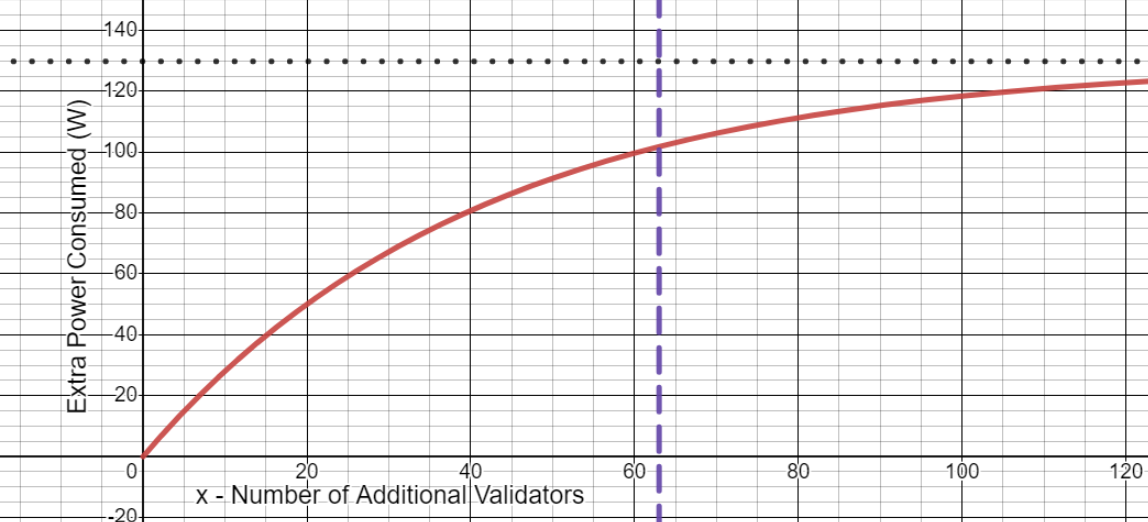
\includegraphics[ width=14cm,center]{Figures/AsymptoteMultipleValidators.png}
    \caption{Graphing \eref{eqn:ExpDecay} showing its inverse exponential decay behaviour, for the hardware configuration 6 example discussed above. The asymptote at $\boldsymbol{\mathrm{A = 129.80}}$W is highlighted by the horizontal dotted (black) line. The dashed vertical (purple) line highlights the value of the curve at $\boldsymbol{\mathrm{x = 63}}$ additional validators to be $\boldsymbol{\mathrm{101.8}}$W.}
    \label{Figure:MultipleValidators}
\end{figure}

\eref{eqn:ExpDecay} is case specific and can be applied independently to estimate the electricity usage of a node with a specific combination of an EL and CL client, as well as a specific hardware configuration. To integrate this equation into the one proposed earlier, \eref{eqn:CCRISync}, it needs to be generalised, keeping all combinations of hardware and clients in mind.

To recapitulate, $\boldsymbol{\mathrm{\overline{V}_{1}}}$ captures the average electricity consumed by a node, running one validator client. 

\begin{equation*}
    \boldsymbol{\mathrm{\overline{V}_{1}} = {\frac{\displaystyle\sum\limits_{i=1}^{n}{ \left({\left(\mathrm{\overline{P}}_{ID} + \mathrm{\overline{P}}_{CL} + \mathrm{\overline{P}}_{EL}\right)} * {\phi_{EL,CL}} \right)}}
{\pi}} }
\end{equation*}

Following this, \eref{eqn:CCRISync} introduced earlier can be re-written as:

\begin{equation*}
     \boldsymbol{\overline{\mathrm{P}}_{SNC} +  \overline{\mathrm{V}}_{1} 
} 
\end{equation*}

When modified to account for $\boldsymbol{\mathrm{x }}$ additional validator clients being run on the same node, it results in 'Model-A' proposed by this study: 

\begin{equation}
\label{eqn:FinalEqnShort}
     \boldsymbol{\mathrm{P}_{SNC} +  \overline{\mathrm{V}}_{1} + \mathrm{\overline{V}(\mathrm{x})}} 
\end{equation}

Which can be expanded to:
\begin{equation*}
     \boldsymbol{\mathrm{P}_{SNC} +  \overline{\mathrm{V}}_{1} + {\left(\mathrm{\overline{P}}_{TDP} -\overline{\mathrm{V}}_{1} )\right(1-\mathrm{e}^{-\mathrm{k}(\mathrm{x})}) \qquad \forall x \in \mathbb{Z}^+}} 
\end{equation*}

Expanding all terms results in the final equation for 'Model-A' to look like:
\begin{align}
\label{eqn:FinalEqnLong}
     &\boldsymbol{({\mathrm{T}_{EL} * ({\mathrm{P}_{TDP}} + \mathrm{P}_{SSD})}) +  {\frac{\displaystyle\sum\limits_{i=1}^{n}{ \left({\left(\mathrm{\overline{P}}_{ID} + \mathrm{\overline{P}}_{CL} + \mathrm{\overline{P}}_{EL}\right)} * {\phi_{EL,CL}} \right)}}
{\pi}}}\nonumber \\  \nonumber\\  
     &\boldsymbol{+ {(\mathrm{\overline{P}}_{TDP} - {\frac{\displaystyle\sum\limits_{i=1}^{n}{ \left({\left(\mathrm{\overline{P}}_{ID} + \mathrm{\overline{P}}_{CL} + \mathrm{\overline{P}}_{EL}\right)} * {\phi_{EL,CL}} \right)}}
{\pi}}} ) (1-\mathrm{e}^{-\mathrm{k}(\mathrm{x})})}\\ \nonumber \\    
     &\boldsymbol{\qquad \qquad \qquad \qquad \qquad \qquad \forall \text{ } x \in \mathbb{Z}^+}\nonumber 
\end{align}

Note that hardware configuration-specific terms, such as the CPU's TDP, SSD's power usage and even electricity measurements for each client, must be weighted by the estimated share of the network using that node hardware in order to get a better estimate for the network's cumulative energy consumption. 

% ___________________________________________________________________MODELS DONE< NOW 

% Model-AAAAAAAAAAAAAAAAAAAAAAAAAAAAAAAAAAAAAAAAAAAAAAAAAA
\section{Results Of Application Of Models And Discussion}
\label{ImplementationSection}
Through extensive data gathering, Model-A, alongside 2 other models from the wider literature, are implemented in this section.


\subsection{Model-A: Implementation}

First, 3 hardware configurations were chosen, including a low, medium and high tier for running Full Nodes. Hardware configurations recommended for running the Geth EL client ($\sim$ 70\% network share) can be found in \tref{Table:RecommendedHardware}.

\begin{table}[htb!]
    \centering
    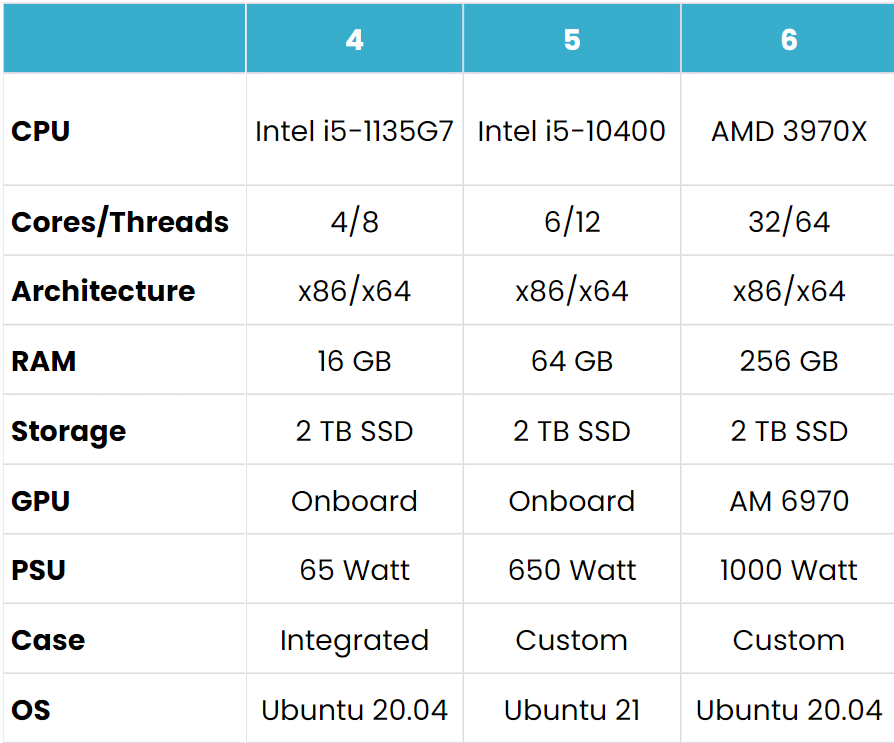
\includegraphics[width=10cm,center]{Figures/CCRIhardwareConfigEdit.png}
    \caption{Adapted from the CCRI report \cite{CryptoCarbonRatingsInstitute2022TheNetwork}, this table shows 3 of the 6 hardware configurations that were used in their experiment detailing a low, mid and high-tier node.}
    \label{Table:CCRIhardwareConfig}
\end{table}

PoS Ethereum was aimed at being run on commodity hardware. Keeping this, as well as the hardware recommendations in \tref{Table:RecommendedHardware} in mind, 3 sets of hardware combinations need to be chosen for implementation of the model. Due to the limited availability of empirical data on hardware running PoS Ethereum, the hardware configurations 4,5 and 6 from \tref{Table:CCRIhardwareConfig} are used. Using this data also helped draw fairer comparisons when evaluating Model-A later on. 

\textbf{Step 1 - Average Sync Energy of a Node}

No empirical data was available for implementing the first part of 'Model-A', \eref{eqn:FinalEqnShort}, denoted by $\boldsymbol{\mathrm{P}_{SNC}}$. Non-scientific data gathered on the synchronisation time $\boldsymbol{\mathrm{T}_{EL}}$, reported by users employing varying combinations of hardware and EL clients, can be found in Appendix B. This data is limited and thus insufficient to differentiate between the sync times for the 4 major EL clients. However, it is sufficient to estimate the average sync time of varying tiers of node hardware (relative to \tref{Table:CCRIhardwareConfig}), presented in \tref{Table:SyncEnergy}. Data collected on hardware running the Geth client was \textbf{assumed} to be more representative and given a higher weighting due to its high network share of $\sim$ 70\%. 

Varying external factors affect a user's decision to choose the appropriate hardware for their node, ranging from different profit structures to low-budget devices and future-proof hardware. There is an immeasurable amount of hardware configurations that users could opt for. Thus, we model this distribution of the 3 categories of node hardware using a continuous distribution, particularly - the CDF (Cumulative distribution function) of the standard normal distribution. This distribution was divided into 3 parts; 25\% of the network is \textbf{assumed} to opt for the low-tier hardware (configuration 4), 50\% for the mid-tier (configuration 5) and 25\% for the high-tier hardware (configuration 6), presented in \tref{Table:SyncEnergy}. 

\begin{table}[h]
\centering
\begin{tabular}{|l|l|l|l|l|}
\hline
\textbf{Tier} & \textbf{$\boldsymbol{\mathrm{T}_{EL}}$ {[}h{]}} & \textbf{$\boldsymbol{\mathrm{P}_{TDP}}$ {[}Wh{]}} & \textbf{$\boldsymbol{\mathrm{P}_{SSD}}$ {[}Wh{]}} & \textbf{Share of the network {[}\%{]}} \\ \hline
Low    & 36 & 28  & 3.5 & 25 \\ \hline
Medium & 24 & 65  & 8.5 & 50 \\ \hline
High   & 12 & 280 & 10  & 25 \\ \hline
\end{tabular}
\caption{Data used to implement the  $\boldsymbol{\mathrm{P}_{SNC}}$ part of 'Model-A'.  $\boldsymbol{\mathrm{P}_{TDP}}$ source: \cite{IntelFAQs}, \cite{AMDDatabase}. $\boldsymbol{\mathrm{P}_{SSD}}$ source: \cite{RachanaKhamamkar2020AnalyzingDrives}.}
\label{Table:SyncEnergy}
\end{table} 

Given \tref{Table:SyncEnergy}, the $\boldsymbol{\mathrm{P}_{SNC}}$ for an average node can be calculated by following its \eref{eqn:Sync}. Each hardware tier's values are multiplied by its network distribution share: 
\begin{align}
    &\boldsymbol{0.25*(36*(28 + 3.5)) + 0.5*(24*(65+8.5)) + 0.25*(12*(280+10))} \nonumber\\ \nonumber \\
    &\boldsymbol{{\mathrm{P}_{SNC}} = 2035.5} \text{ Wh per node} \nonumber
\end{align}

% ________________________________________--

% _---------------------------------------
\textbf{Step 2 - Average electricity consumption of a node bar sync energy}
\label{postSyncEnergyImplementation}

The next part of \eref{eqn:FinalEqnShort}, $\boldsymbol{\mathrm{\overline{V}_{1}}}$ needs to be implemented. \tref{Table:ClientShares} presents contemporary data collected for each EL and CL client's shares of the Ethereum network, required to calculate $\boldsymbol{\phi_{EL,CL}}$.  

% --------------------------------------
\begin{table}[h]
    \centering

  \subcaptionbox{\textbf{Execution Clients} \cite{Sigp/blockprint:Metrics}}{
      \begin{tabular}{|l|c|}
            \hline
             Geth & 69.22 \% \\
            \hline
             Nethermind & 14.16 \%  \\
            \hline 
             Erigon & 10.65 \% \\
            \hline
             Besu & 5.78 \% \\
            \hline
             OpenEthereum & 0.00 \% \\
            \hline
             Other & 0.20 \% \\
            \hline
  \end{tabular}
    \label{Table:ClientShares:left}
  }
  \subcaptionbox{\textbf{Consensus Clients}  \cite{ClientsExplorer}}{
        \begin{tabular}{|l|c|}
                    \hline
             Prysm & 65.15 \%  \\
            \hline
             Lighthouse & 29.30 \% \\
            \hline 
             Teku & 10.65 \% \\
            \hline
             Nimbus & 0.91 \% \\
            \hline
             Lodestar & 0.0 \% \\
            \hline
             Other & 0.0 \%  \\
            \hline
            
  \end{tabular}
    \label{Table:ClientShares:right}
  }
    \caption{An updated table of client diversity within Ethereum Mainnet network, data recorded on 27-Mar 23. Updates table 5 from report \cite{CryptoCarbonRatingsInstitute2022TheNetwork} }
  \label{Table:ClientShares}
\end{table}

% --------------------------------------------


Empirical data on the energy consumption values recorded for all 3 hardware configurations running all clients separately can be found in \tref{Table:ConsumptionValues}. The Nethermind client which now holds a sizeable network share has no empirical energy consumption data available. Its values are substituted by the other 3 EL clients' averaged values per configuration.

% ----------------------
\begin{table}[htb!]
\centering
\begin{tabular}{|l|lll|}
\hline
\textbf{Client Name} & \multicolumn{3}{l|}{\textbf{Node Configuration}}                               \\ \hline
\textbf{}            & \multicolumn{1}{l|}{\textbf{4}} & \multicolumn{1}{l|}{\textbf{5}} & \textbf{6} \\ \thickhline
Idle Node (No Client)               & \multicolumn{1}{l|}{3.66}       & \multicolumn{1}{l|}{25.04}      & 78.17      \\ \cline{1-1}
Geth (EL)            & \multicolumn{1}{l|}{11.23}      & \multicolumn{1}{l|}{9.70}       & 47.70      \\ \cline{1-1}
Erigon (EL)          & \multicolumn{1}{l|}{18.60}      & \multicolumn{1}{l|}{17.59}      & 44.62      \\ \cline{1-1}
Besu (EL)            & \multicolumn{1}{l|}{30.25}      & \multicolumn{1}{l|}{31.02}      & 75.04      \\ \cline{1-1}
Nethermind(EL)[Averaged] & \multicolumn{1}{l|}{20.03}       & \multicolumn{1}{l|}{19.44}       & 55.79      \\ \cline{1-1}
Prysm (CL)           & \multicolumn{1}{l|}{3.51}       & \multicolumn{1}{l|}{2.87}       & 24.33      \\ \cline{1-1}
Lighthouse (CL)      & \multicolumn{1}{l|}{2.75}       & \multicolumn{1}{l|}{3.14}       & 18.84      \\ \cline{1-1}
Teku (CL)            & \multicolumn{1}{l|}{3.71}       & \multicolumn{1}{l|}{3.32}       & 27.46      \\ \cline{1-1}
Nimbus (CL)          & \multicolumn{1}{l|}{1.67}       & \multicolumn{1}{l|}{2.08}       & 17.11      \\ \cline{1-1}
Lodestar(CL)         & \multicolumn{1}{l|}{3.14}       & \multicolumn{1}{l|}{3.89}       & 33.55      \\ \hline

\end{tabular}
\caption{Mean electricity consumption values [in Wh] measured in the report \cite{CryptoCarbonRatingsInstitute2022TheNetwork} for hardware configurations 4-6 mentioned in \tref{Table:CCRIhardwareConfig} running various clients.  }
\label{Table:ConsumptionValues}
\end{table}

Given the data in \tref{Table:ConsumptionValues}, values in \tref{Table:EstimatesPerNode} were be calculated. For example, the first row (Prysm,Geth) was calculated by adding the electricity usage when idle, running Pyrsm, and running Geth per configuration, multiplied by its hardware tier distribution across the network, shown below:
\begin{align}
    &\boldsymbol{0.25*(3.66 + 11.23 + 3.51) + 0.50 * (25.04 + 9.70 + 2.87) + 0.25} \nonumber\\
    &\boldsymbol{* (78.17 + 47.70 + 24.33) = 60.96}\text{Wh} \nonumber
\end{align}

% -----------------------------------------
\begin{table}[htb!]
\centering
\begin{tabular}{|ll|l|l|l|}
\hline
\multicolumn{2}{|l|}{\textbf{Client Combination}} &
  \multirow{2}{*}{\textbf{\begin{tabular}[c]{@{}l@{}}Estimate\\ {[}Wh{]}\end{tabular}}} &
  \multirow{2}{*}{\textbf{\begin{tabular}[c]{@{}l@{}}Annualised Estimate\\ {[}kWh/year{]}\end{tabular}}} &
  \multirow{2}{*}{\textbf{\begin{tabular}[c]{@{}l@{}}Client Combination\\ Share {[}\%{]}\end{tabular}}} \\ \cline{1-2}
\multicolumn{1}{|l|}{\textbf{CL Client}} & \textbf{EL Client} &       &        &       \\ \hline
\multicolumn{1}{|l|}{Prysm}              & Geth               & 60.96 & 533.97 & 45.10 \\ \cline{1-2}
\multicolumn{1}{|l|}{Prysm}              & Erigon             & 65.97 & 577.91 & 6.94  \\ \cline{1-2}
\multicolumn{1}{|l|}{Prysm}              & Besu               & 83.21 & 728.88 & 3.77  \\ \cline{1-2}
\multicolumn{1}{|l|}{Prysm}              & Nethermind         & 70.05 & 613.62 & 9.23  \\ \cline{1-2}
\multicolumn{1}{|l|}{Lighthouse}         & Geth               & 59.53 & 521.47 & 20.28 \\ \cline{1-2}
\multicolumn{1}{|l|}{Lighthouse}         & Erigon             & 64.54 & 565.41 & 3.12  \\ \cline{1-2}
\multicolumn{1}{|l|}{Lighthouse}         & Besu               & 81.78 & 716.38 & 1.69  \\ \cline{1-2}
\multicolumn{1}{|l|}{Lighthouse}         & Nethermind         & 68.62 & 601.11 & 4.15  \\ \cline{1-2}
\multicolumn{1}{|l|}{Teku}               & Geth               & 62.01 & 543.24 & 7.37  \\ \cline{1-2}
\multicolumn{1}{|l|}{Teku}               & Erigon             & 67.03 & 587.18 & 1.13  \\ \cline{1-2}
\multicolumn{1}{|l|}{Teku}               & Besu               & 84.26 & 738.15 & 0.62  \\ \cline{1-2}
\multicolumn{1}{|l|}{Teku}               & Nethermind         & 71.11 & 622.88 & 1.51  \\ \cline{1-2}
\multicolumn{1}{|l|}{Nimbus}             & Geth               & 58.29 & 510.66 & 0.63  \\ \cline{1-2}
\multicolumn{1}{|l|}{Nimbus}             & Erigon             & 63.31 & 554.59 & 0.10  \\ \cline{1-2}
\multicolumn{1}{|l|}{Nimbus}             & Besu               & 80.54 & 705.57 & 0.05  \\ \cline{1-2}
\multicolumn{1}{|l|}{Nimbus}             & Nethermind         & 67.39 & 590.31 & 0.13  \\ \hline
\end{tabular}
\caption{Electricity consumption estimates (best guess) per node for all possible client combinations. Used to calculate $\boldsymbol{\mathrm{\overline{V}_{1}}}$.  }
\label{Table:EstimatesPerNode}
\end{table}

% -----------------------------------
Following \eref{eqn:CCRI}, best guess for an individual node =  \textbf{63.76 Wh}. This can be annualised (8760h in a year) = \textbf{558.55 kWh/year}.

\textbf{Assuming} the node needs to perform a fresh synchronisation once a year, the annual total consumption of an average node (running 1 validator):

\begin{align}
    &\boldsymbol{ \mathrm{\overline{V}_{1}} + \mathrm{P}_{SNC} = \text{560.58 kWh/year or 63.99 Wh.}} \nonumber
\end{align} 

% --------------------------------------------------
% STAGE 3 of implementation with multiple validators
% --------------------------------------------------
\textbf{ Step 3 - Running multiple validators on some nodes}

Implementing the final part of \eref{eqn:FinalEqnShort}, $\boldsymbol{\mathrm{\overline{V}(\mathrm{x})}}$, accounts for some nodes running multiple validators. 

When users operate additional validator clients, they often run a 1000+ to take advantage of the exponential decrease in energy consumption, seen in \sref{AdditonalNodesReasoning}. Currently, there are 561,472 validators running. Based on this, and for the sake of simplicity, it can be \textbf{assumed} that 1000 additional validators are run on $\sim$562 nodes (of the total $\sim$12000 network nodes), running on mid to high-tier hardware. Thus, following \eref{eqn:Sync} yields:

$\boldsymbol{\mathrm{\overline{P}}_{TDP}}$ (from \tref{Table:SyncEnergy}): \textbf{205 Wh} \\
$\boldsymbol{ \overline{\mathrm{V}}_{1}}$ (from \sref{postSyncEnergyImplementation}) : \textbf{63.99 Wh} 

$\boldsymbol{\mathrm{k}}$ can be calculated by the method shown in the example in \sref{DetermineK}:

\begin{equation*}
    \boldsymbol{\mathrm{141.01} * (1-\mathrm{e}^{-\mathrm{k}(\mathrm{63})}) = \mathrm{120.51}}
\end{equation*}

Which solves to:
\begin{equation*}
    \boldsymbol{\mathrm{k} = \mathrm{{3.061} * {10}^{-2}}}
\end{equation*}

Once $\boldsymbol{\mathrm{k}}$ has been calculated, $\boldsymbol{\mathrm{x}}$ can be set to \textbf{1000} additional validators for 562 of the total nodes on the network while the rest run no additional nodes.
\begin{center}
    $\boldsymbol{\mathrm{\overline{V}(\mathrm{1000})}} =$ \textbf{141.10 Wh} \\
 \textbf{141.10 $*$ 562 = 79.29 kWh}
\end{center}

The new hourly consumption of the entire network: \textbf{862.66 kWh}. Final results are compiled in \tref{Table:FinalResults}.
% The new hourly energy consumption of a single node can be derived: \textbf{70.47} Wh
% Annual energy consumption of a single node: 617.30 kWh 
% Annual energy consumption of the network: 7.5569 GWh
% Annual energy consumption of a single node per transaction: 0.0015738 Wh/tx
% Annual energy consumption of the network per transaction: 19.27 Wh/tx



% ____________________________________________________________________________
% \subsubsection{Additonal Assumptions}
% \label{Assumptions}

% \begin{itemize}
    % \item They have taken the syncing on nodes into account into their model whereas for general modelling, it would be  abetter estimate to ignore this initial set up energy and get an avergae form then on. That is what this paper has done, taking averages of the Raspberry Pi rather than including the syncing energy.
    % \item The TDP + SSD power usage can be used as an upper limit for the energy consumption of any hardware set-up
    % \item That growth for more than one validator can be modelled by an exponential decay (increasing form)
    % \item This exponential growth has an upper limit of TDP + SSD power usage and using the single validator energy consumption as the lower limit
%     \item The CCRI model has been verified and is accurate. Thus it is acceptable to use as the base for 'Model-A'
%     \item The EL and CL clients are not changed; just additional Validator clients are run on the same set up
%     \item 10\% lower than the TDP power should be reached by the time the 64$^\mathrm{{th}}$ validator is run.
%     \item Took averages of other EL layer clients per confirguration for NetherMind. not good.
%     \item All these numbers are for running a full node, not validators which sdmieler,2020 said is basically negligible
%     \item high, mid low tiers dont have a fair distribution of hardware but does help achieve more accurate results hopefully
%     \item for table \_\_ gave higher importance to Geth to estimate sync time as it has a much larger share of the network than the other EL clients
% \end{itemize}

\subsection{Implementing Competing Models}

As mentioned in \sref{LitRevExistingModels} there are two existing models found in the wider literature. 

\textbf{The CCRI Model} 

This model \cite{CryptoCarbonRatingsInstitute2022TheNetwork} forms the $ \boldsymbol{\overline{\mathrm{V}}_{1}}$ part of Model-A proposed in this study, detailed in \sref{CCRIBaseEqnSection}. Through the implementation of Model-A, the CCRI model was also implemented as a step. All the contemporary data collected in \tref{Table:ClientShares} and \tref{Table:ConsumptionValues} was used for calculations in \tref{Table:EstimatesPerNode}. Ever since the CCRI report, OpenEthereum has been deprecated, and the Lodestar client no longer holds a sizeable share of the network, and they were not included in calculations. The study splits the network share between the 3 hardware tiers (low, mid and high-tier) binomially rather than using a continuous distribution like this study. However, the split remains the same at 25\%, 50\%, and 25\%, respectively, making the results more comparable. The final results from this model can be found in \tref{Table:FinalResults}.

\textbf{The UCL Model} 

The original UCL model can be found in report \cite{Platt2022TheProof-of-Work}. It was recently updated on 7$\mathrm{^{th}}$ Feb 2023 \cite{IbanezTheExpansion}, and contemporary results from the updated report are directly taken and updated with the same metrics used to implement Model-A for a fair comparison. Results can be found in \tref{Table:FinalResults}. 


\subsection{Final Results}
\label{ResultsSection}
Metrics recorded on 10$\mathrm{^{th}}$ April 2023: \\
Number of nodes connected to Ethereum mainnet: \textbf{12242 nodes} \cite{NodewatchAnalytics} \\
Number of transactions completed each day: \textbf{1074596 tx/day}  \cite{EthereumBlockchair} \\
The number of validators on the network: \textbf{562729 validators} 
\cite{EthereumEthereum.orgc}

Using these metrics, results for each of the aforementioned models are presented in \tref{Table:FinalResults}.
\clearpage
% -----------------------------------------------
% RESULTS  TABLEEEE
% ----------------------------------------------------------------
\begin{table}[h]
\begin{tabular}{ll"ll"l"l|}
\cline{3-6}
 &
   &
  \multicolumn{2}{l"}{\textbf{Model-A}} &
  \textbf{CCRI \cite{CryptoCarbonRatingsInstitute2022TheNetwork}} &
  \textbf{UCL \cite{IbanezTheExpansion}} \\ \thickhline
\multicolumn{1}{|l|}{\multirow{2}{*}{\textbf{\begin{tabular}[c]{@{}l@{}}Accounts \\ For:\end{tabular}}}} &
  \textbf{\begin{tabular}[c]{@{}l@{}}Synchronisation \\ Energy \end{tabular}} &
  \multicolumn{1}{l|}{Yes} &
  Yes &
  No &
  No \\ \cline{2-6} 
\multicolumn{1}{|l|}{} &
  \textbf{\begin{tabular}[c]{@{}l@{}}Additional Validators \\ Per Node\end{tabular}} &
  \multicolumn{1}{l|}{No} &
  Yes &
  No &
  No \\ \hline
\multicolumn{1}{|l|}{\multirow{2}{*}{\textbf{Hourly}}} &
  \textbf{\begin{tabular}[c]{@{}l@{}}Per Node \\ {[}Wh{]}\end{tabular}} &
  \multicolumn{1}{l|}{63.99} &
  70.47 &
  63.76 &
  85.03 \\ \cline{2-6} 
\multicolumn{1}{|l|}{} &
  \textbf{\begin{tabular}[c]{@{}l@{}}Entire Network \\ {[}kWh{]}\end{tabular}} &
  \multicolumn{1}{l|}{783.37} &
  862.66 &
  780.57 &
  1040.09 \\ \hline
\multicolumn{1}{|l|}{\multirow{4}{*}{\textbf{Annual}}} &
  \textbf{\begin{tabular}[c]{@{}l@{}}Per Node \\ {[}kWh{]}\end{tabular}} &
  \multicolumn{1}{l|}{560.58} &
  617.30 &
  558.55 &
  744.86 \\ \cline{2-6} 
\multicolumn{1}{|l|}{} &
  \textbf{\begin{tabular}[c]{@{}l@{}}Entire Network \\ {[}GWh{]}\end{tabular}} &
  \multicolumn{1}{l|}{6.86} &
  7.56 &
  6.84 &
  9.12 \\ \cline{2-6} 
\multicolumn{1}{|l|}{} &
  \textbf{\begin{tabular}[c]{@{}l@{}}Per Node / Transaction \\ {[}mWh/tx{]}\end{tabular}} &
  \multicolumn{1}{l|}{1.43} &
  1.57 &
  1.42 &
  1.90 \\ \cline{2-6} 
\multicolumn{1}{|l|}{} &
  \textbf{\begin{tabular}[c]{@{}l@{}}Entire Network / Transaction \\ {[}Wh/tx{]}\end{tabular}} &
  \multicolumn{1}{l|}{17.50} &
  19.27 &
  17.43 &
  23.25 \\ \hline
\end{tabular}
\caption{Best guess estimates obtained by implementing 'Model-A' as well as 2 other models, all using the same metrics introduced earlier.}
\label{Table:FinalResults}
\end{table}
% -----------------------------------------------------------------------

% ______________________________________________________________________
% \section {Modelling Ethereum's Carbon Emissions}
% \url{https://ethernodes.org/countries}

% \paragraph{ Simple Linear Regression Model}
% A simple logical model for estimating the energy consumption of Ethereum 2.0's energy consumption logically would be using simple regression. y = mx + c, and if we wanted to say that energy is dependent on transactions, then we can say y is the energy per node, m is the slope we need to find, x is the number of transactions/sec, c is the base energy an idle node requires. Then we multiply this whole thing by the number of validators on the network to get the overall network energy consumption.

% _____________________________________________________________________________
% _____________________________________________________________________________
% ____________________________________________________________________________
\section{Evaluation and Discussion}

\subsection{Interpretation}

Being able to model the electricity consumption of PoS Ethereum successfully answers RQ1. The results produced by Model-A are valid due to three main reasons:
\begin{enumerate}
    \item The qualitative criteria defined in \sref{QualModelEvalMEthodology}, for model formulation to be valid, has been met. 
    \begin{itemize}
        \item Credible sources have been used to justify each assumption and conclusion drawn during the formulation of Model-A. Comprehensive documentation of each justification has been provided, and all 8 assumptions have been emphasised in the text using bold formatting.
        \item All data utilised in the modelling process were either derived from strictly empirical sources or an average of a comprehensive collection of non-scientific sources.
    \end{itemize}
    \item Model-A's results fall between the only two other models found in the wider literature, thus positioning them within a 'reasonable' range.
    \item A In accordance with the quantitative evaluation criteria defined in \sref{MethoologyErrorQuant}, for the results to be deemed satisfactory, $\boldsymbol{\epsilon_\mathrm{rme} \leq 0.2}$. By treating the experimentally verified CCRI model's results as true values and comparing the energy consumption for the entire network per transaction, the $\boldsymbol{\epsilon_\mathrm{rme} = 7.96 * 10^{-2}}$ is obtained, making it acceptable.   
\end{enumerate}

Model-A accounts for 2 more sources of energy expenditure as compared to the base CCRI model, which explains the average Percentage Increase (PE) of 9.5\% across all values. 9.25\% of it can be attributed to operating additional validators, suggesting that the extra energy consumed by accounting for $\sim$500000 extra validators was weighted reasonably since it didn't have a disproportionate effect on our final results. 

The UCL model seems to overestimate consumption values. This may stem from the model's lack of complexity, which is a consequence of its generalisation to encompass six PoS blockchains.

\begin{figure}[!htb]
    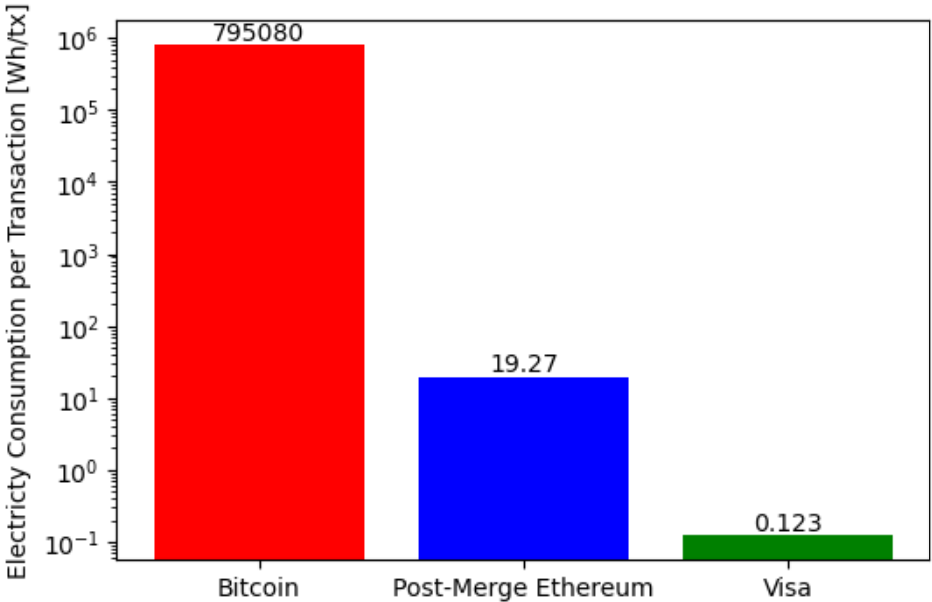
\includegraphics[width=13cm,center]{Figures/ElectricityConsumptionPlot.png}
    \caption{2022 data on electricity consumption per transaction for Bitcoin \cite{BitcoinDigiconomist}, Ethereum 2.0 [from Model-A] and Visa \cite{2022VisaReport}, \cite{VisaHome} plotted on a logarithmic scale. Code available in Appendix C}
    \label{Figure:ElectricityConsumptionPlot}
\end{figure}

PoS Ethereum has had a reduction of 99.997\% in its overall energy use when compared to PoW Ethereum's consumption average over 2022, going from 24.99TWh/year to 7.56kWh/year according to Model-A(\cite{CCRIIndices}). This answers RQ2 (\sref{ResearchQuestions}) - the claimed energy reduction of 99.988\% is only inaccurate by less than 0.01\% according to Model-A, as shown in \fref{Figure:PaypalEthElectrcityPlot}.

According to \fref{Figure:ElectricityConsumptionPlot}, Visa can process 
$\sim$156 transactions in the same amount of energy it takes PoS Ethereum to complete a single one. This often-made comparison is not one that is fair to make. Ethereum is a completely self-contained monetary system, whereas Visa relies on a range of intermediaries such as the global banking system, SWIFT and the diplomatic strength of the U.S. government \cite{Carter2021BitcoinComparison}. It is like comparing apples to kangaroos. Instead, Ethereum should be compared to Paypal, a platform that, along with digital payments, also offers other financial services and bank-like services.  

\begin{figure}[!htb]
    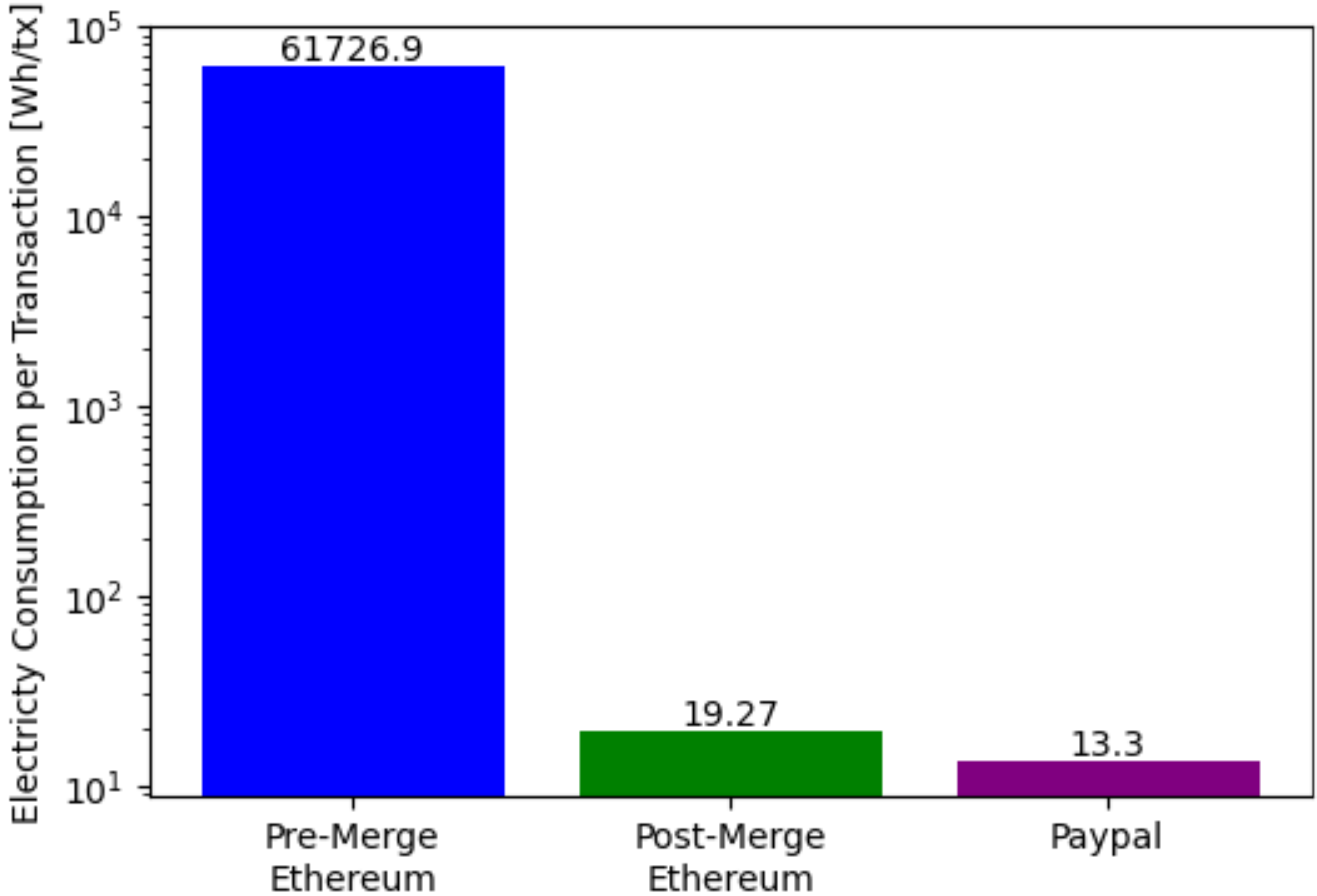
\includegraphics[width=13cm,center]{Figures/PaypalEthElectrcityPlot.png}
    \caption{Electricity consumption per transaction for Ethereum 1.0 \cite{CCRIIndices}, \cite{EthereumBlockchair}, Ethereum 2.0 [from Model-A] and Paypal \cite{2007IntroductionPayPal}. Code found in Appendix C.}
    \label{Figure:PaypalEthElectrcityPlot}
\end{figure}

\fref{Figure:PaypalEthElectrcityPlot} shows that Ethereum 2.0 is impressively close to Paypal's energy consumption while maintaining decentralisation, according to Model-A.



% ____________________________________________________________________________
\subsection{Limitations and Future Work}
\label{LimitationsFutureWork}

\textbf{Secondary data:} Data from the scientific experiment performed in the CCRI report \cite{CryptoCarbonRatingsInstitute2022TheNetwork} was used as it measured the precise metrics needed for this study. First-hand data collection was out of the scope of this study as the hardware required for mid and high-tier configurations would've cost $\sim$£2500 while also requiring 23 days of simultaneously running all 3 nodes. However, no validator nodes were run in the experiment as staking 32ETH was infeasible and the additional electricity was viewed as negligible. While we have disproven this assumption by modelling data found from consistent but non-scientific sources, more work is needed on studying the effects of overloading nodes with thousands of additional validators. Moreover, the impact of this workload on different hardware configurations should also be considered so fewer assumptions are made. 

\textbf{Lack of data:} Due to the innovative nature of the research being conducted, there was a paucity of data available for analysis. Some of the improvements made upon the base model come from modelling non-scientific data; hence the model was implemented on averaged values to obtain a 'best guess' estimation. Through further scientific experimentation, high and low estimates can be found to obtain a range that the final results should lie within. 

\textbf{Energy inefficiencies: } Electricity consumption data comes from monitoring software run on computers. Thus, these are not 'at-wall' values which truly show how much electricity is being drawn from the national grid, possibly due to voltage regulators that limit the power supply to the machine. This model could benefit from further work conducted by individuals well versed in electrical engineering that account for this dissipated energy, obtaining a more accurate estimation 'At-wall' \cite{Warkozek2012ACenters}.

\textbf{Simulation and Prediction: } There is potential for future work in creating a computer-based simulation of this model or just on existing blockchain benchmarking software such as Hyperledger Caliper or Blockbench \cite{Aldweesh2020BenchmarkingApplications}. A more ambitious goal would be predicting energy consumption given different values for the factors included in the model, which would require curve-fitting \cite{IbanezTheExpansion}.

% _______________________________________________________________________

\setcounter{chapter}{5}
% \chapter{Use Case: Drug Supply Chain Decentralisation}
% \section{Chapter Summary}
% \section{Introduction}
% \section{A Brief Literature Review}
% \subsection{Pain Points in Drug Supply Chains}
% \subsection{Corresponding Benefits of Blockchain Solutions}
% \subsection{Proposed Implementations In the Literature}
% \section{Contextualising Our Energy Model}
% \section{Limitations And Future Work}
% \section{Key Points Covered}


% __________________________________________________________________APPENDIX
\appendix
\chapter{Validator Hardware Data}

Data gathered on the hardware configurations reported by users across various sources has been collected in the tables \tref{Table:HardwareTable1} and \tref{Table:HardwareTable2} below.

% ___________________________________
\begin{landscape}
\begin{table}[]
\centering
\begin{tabular}{@{}|l|l|l|l|l|l|l|@{}}
\toprule
\textbf{No.} & \textbf{Source} & \textbf{Name}                                                                               & \textbf{Specification}                                                                                                            & \textbf{Clients}                                             & \textbf{Usage per hour}                                     & \textbf{Link}                                         \\ \midrule
1            & Scientific          & \begin{tabular}[c]{@{}l@{}}Recommended Specs \\ for Solo Validator\end{tabular}             & \begin{tabular}[c]{@{}l@{}}Quad Core or Dual Core \\ Hyperthreaded Processor, \\ 2TB SSD , \textgreater{}16GB memory\end{tabular} & Any                                                          & NA                                                          & \cite{2022DeveloperGo-ethereum} \\ \midrule
2            & Scientific         & \begin{tabular}[c]{@{}l@{}}Recommended Specs \\ for Archive Nodes\end{tabular}              & \begin{tabular}[c]{@{}l@{}}Quad Core or Dual Core \\ Hyperthreaded Processor, \\ 12TB SSD, \textgreater{}16GB memory\end{tabular} & Any                                                          & NA                                                          & \cite{2022DeveloperGo-ethereum} \\ \midrule
3            & Scientific          & \begin{tabular}[c]{@{}l@{}}Minimum Recommended \\ Specs for Validator nodes\end{tabular}    & \begin{tabular}[c]{@{}l@{}}Dual Core Hyperthreaded, \\ 1TB SSD, \textgreater{}4GB memory\end{tabular}                             & Any                                                          & NA                                                          & \cite{2022DeveloperGo-ethereum}\\ \midrule
4            & Non-Scientific          & Solo Validator                                                                              & NUC Intel i5 11th Gen                                                                                                             & \begin{tabular}[c]{@{}l@{}}Lighthouse + \\ Besu\end{tabular} & \begin{tabular}[c]{@{}l@{}}40Wh \\ upper limit\end{tabular} & \cite{EnergyEthstakerb}              \\ \midrule
5            & Non-Scientific          & Low Power Solo Validator                                                                    & Raspberry Pi 4                                                                                                                    & \begin{tabular}[c]{@{}l@{}}Nimbus + \\ Geth\end{tabular}     & 8Wh                                                         & \cite{EnergyEthstakerb}              \\ \midrule
6            & Non-Scientific          & Low Power Solo Validator                                                                    & Raspberry Pi 4                                                                                                                    & \begin{tabular}[c]{@{}l@{}}Prysm \\ + Geth\end{tabular}      & 9Wh                                                         & \cite{EnergyEthstakerb}              \\ \midrule
7            & Non-Scientific          & \begin{tabular}[c]{@{}l@{}}Average Energy Usage for \\ Solo Validators on NUCs\end{tabular} & Mid Spec NUC                                                                                                                      & Any                                                          & 15-20Wh                                                     & \cite{EnergyEthstakerb}              \\ \bottomrule
\end{tabular}
\caption{Data on various validator node hardware configurations and their energy consumption. Continued in \tref{Table:HardwareTable2}.}
\label{Table:HardwareTable1}
\end{table}
\end{landscape}
% ____________________________________
\begin{landscape}
\begin{table}[]
\centering
\begin{tabular}{|l|l|l|l|l|l|l|}
\hline
\textbf{No.} & \textbf{Source Type} & \textbf{Name}                                                                  & \textbf{Specification}                                                     & \textbf{Clients}                                             & \textbf{Usage per hour}                                    & \textbf{Link} \\ \hline
8            & Non-Scientific          & Solo Validator                                                                 & \begin{tabular}[c]{@{}l@{}}Asus PN50 mini PC, \\ Ryzen 4800 U\end{tabular} & \begin{tabular}[c]{@{}l@{}}Lighthouse + \\ Besu\end{tabular} & \begin{tabular}[c]{@{}l@{}}10.45Wh \\ At-wall\end{tabular} & \cite{EnergyEthstakerb}           \\ \hline
9            & Non-Scientific          & \begin{tabular}[c]{@{}l@{}}Multiple Validators on \\ high end PCs\end{tabular} & Alienware Aurora                                                           & Unknown                                                      & 2 Wh                                                       & \cite{EnergyEthstakerb}           \\ \hline
10           & Non-Scientific          & NUC Validator                                                                  & General NUC                                                                & Unknown                                                      & 18.4Wh                                                     & \cite{EnergyEthstakerb}           \\ \hline
11           & Non-Scientific          & Solo Validator                                                                 & NUC Intel i7 10th Gen                                                      & \begin{tabular}[c]{@{}l@{}}Teku +\\  Besu\end{tabular}       & 15Wh                                                       & \cite{EnergyEthstakerb}           \\ \hline
12           & Non-Scientific          & Solo Validator                                                                 & NUC 10 Intel i5                                                            & \begin{tabular}[c]{@{}l@{}}Teku + \\ Geth\end{tabular}       & 20.83Wh                                                    & \cite{EnergyEthstakerb}           \\ \hline
13           & Non-Scientific          & Solo Validator PC                                                              & \begin{tabular}[c]{@{}l@{}}Ryzen 5, 2TB SSD, \\ 32GB memory\end{tabular}   & Unknown                                                      & 28Wh                                                       & \cite{EnergyEthstakerb}           \\ \hline
14           & Non-Scientific          & Solo Validator PC                                                              & \begin{tabular}[c]{@{}l@{}}ASUS pn50 \\ Ryzen 4300u\end{tabular}           & Unknown                                                      & 8.33Wh                                                     & \cite{EnergyEthstakerb}           \\ \hline
15           & Non-Scientific          & 1000s of Validators                                                            & General NUC                                                                & \begin{tabular}[c]{@{}l@{}}Prysm + \\ Geth\end{tabular}      & \begin{tabular}[c]{@{}l@{}}150Wh \\ upper lim\end{tabular} & \cite{EnergyEthstaker}          \\ \hline
\end{tabular}
\caption{Continuation of \tref{Table:HardwareTable1}. Data on various validator node hardware configurations and their energy consumption.}
\label{Table:HardwareTable2}
\end{table}
\end{landscape}


\chapter{Node Synchronisation Time Data}

\tref{Table:ELRunTime} compiles data collected on the amount of time it takes for various clients to complete the synchronisation process. 

\begin{table}[htb!]
\centering
\begin{tabular}{|l|l|l|l|l|l|}
\hline
\textbf{Client Name} & \textbf{Sync Type} & \textbf{Time} & \textbf{Hardware Tier} & \textbf{Source Type} & \textbf{Source} \\ \hline
Nethermind & Fast & 20h    & Unspecified & Official   & \cite{2022SyncDocs} \\ \hline
Nethermind & Snap & 16h    & Unspecified & Unofficial & \cite{3Ethstakerc} \\ \hline
Geth       & Full & 12-24h & Unspecified & Unofficial & \cite{3Ethstakerb} \\ \hline
Erigon     & Full & 6d 4h  & Mid         & Unofficial & \cite{3Ethstaker}  \\ \hline
Erigon     & Full & 6d     & Low         & Official   & \cite{2022Ledgerwatch/erigon:Frontier}  \\ \hline
Erigon     & Full & 5d     & Medium      & Official   & \cite{2022Ledgerwatch/erigon:Frontier}  \\ \hline
Erigon     & Full & 4d     & High        & Official   &\cite{2022Ledgerwatch/erigon:Frontier} \\ \hline
Besu       & Fast & 1.5d   & Medium      & Official   & \cite{SyncBesu} \\ \hline
Besu       & Snap & 6h     & Medium      & Official   & \cite{SyncBesu} \\ \hline
\end{tabular}
\caption{Data on synchronisation times for all EL clients being run on various hardware configuration tiers relative to \fref{Figure:CCRIhardwareConfig} .}
\label{Table:ELRunTime}
\end{table}


% ---------------
\backmatter
\bibliographystyle{IEEEtranN}
\bibliography{references}
\chapter{Appendix}

\section{Validator Hardware Data}
Data gathered on the hardware configurations reported by users across various sources has been collected in the tables \tref{Table:HardwareTable1} and \tref{Table:HardwareTable2} below.

% ___________________________________
\begin{landscape}
\begin{table}[]
\centering
\begin{tabular}{@{}|l|l|l|l|l|l|l|@{}}
\toprule
\textbf{No.} & \textbf{Source} & \textbf{Name}                                                                               & \textbf{Specification}                                                                                                            & \textbf{Clients}                                             & \textbf{Usage per hour}                                     & \textbf{Link}                                         \\ \midrule
1            & Go-Eth          & \begin{tabular}[c]{@{}l@{}}Recommended Specs \\ for Solo Validator\end{tabular}             & \begin{tabular}[c]{@{}l@{}}Quad Core or Dual Core \\ Hyperthreaded Processor, \\ 2TB SSD , \textgreater{}16GB memory\end{tabular} & Any                                                          & NA                                                          & \cite{2022DeveloperGo-ethereum} \\ \midrule
2            & Go- Eth         & \begin{tabular}[c]{@{}l@{}}Recommended Specs \\ for Archive Nodes\end{tabular}              & \begin{tabular}[c]{@{}l@{}}Quad Core or Dual Core \\ Hyperthreaded Processor, \\ 12TB SSD, \textgreater{}16GB memory\end{tabular} & Any                                                          & NA                                                          & \cite{2022DeveloperGo-ethereum} \\ \midrule
3            & Go-Eth          & \begin{tabular}[c]{@{}l@{}}Minimum Recommended \\ Specs for Validator nodes\end{tabular}    & \begin{tabular}[c]{@{}l@{}}Dual Core Hyperthreaded, \\ 1TB SSD, \textgreater{}4GB memory\end{tabular}                             & Any                                                          & NA                                                          & \cite{2022DeveloperGo-ethereum}\\ \midrule
4            & Reddit          & Solo Validator                                                                              & NUC Intel i5 11th Gen                                                                                                             & \begin{tabular}[c]{@{}l@{}}Lighthouse + \\ Besu\end{tabular} & \begin{tabular}[c]{@{}l@{}}40Wh \\ upper limit\end{tabular} & \cite{EnergyEthstakerb}              \\ \midrule
5            & Reddit          & Low Power Solo Validator                                                                    & Raspberry Pi 4                                                                                                                    & \begin{tabular}[c]{@{}l@{}}Nimbus + \\ Geth\end{tabular}     & 8Wh                                                         & \cite{EnergyEthstakerb}              \\ \midrule
6            & Reddit          & Low Power Solo Validator                                                                    & Raspberry Pi 4                                                                                                                    & \begin{tabular}[c]{@{}l@{}}Prysm \\ + Geth\end{tabular}      & 9Wh                                                         & \cite{EnergyEthstakerb}              \\ \midrule
7            & Reddit          & \begin{tabular}[c]{@{}l@{}}Average Energy Usage for \\ Solo Validators on NUCs\end{tabular} & Mid Spec NUC                                                                                                                      & Any                                                          & 15-20Wh                                                     & \cite{EnergyEthstakerb}              \\ \bottomrule
\end{tabular}
\caption{Data on various validator node hardware configurations and their energy consumption. Continued in \tref{Table:HardwareTable2}.}
\label{Table:HardwareTable1}
\end{table}
\end{landscape}
% ____________________________________
\begin{landscape}
\begin{table}[]
\centering
\begin{tabular}{|l|l|l|l|l|l|l|}
\hline
\textbf{No.} & \textbf{Source} & \textbf{Name}                                                                  & \textbf{Specification}                                                     & \textbf{Clients}                                             & \textbf{Usage per hour}                                    & \textbf{Link} \\ \hline
8            & Reddit          & Solo Validator                                                                 & \begin{tabular}[c]{@{}l@{}}Asus PN50 mini PC, \\ Ryzen 4800 U\end{tabular} & \begin{tabular}[c]{@{}l@{}}Lighthouse + \\ Besu\end{tabular} & \begin{tabular}[c]{@{}l@{}}10.45Wh \\ At-wall\end{tabular} & \cite{EnergyEthstakerb}           \\ \hline
9            & Reddit          & \begin{tabular}[c]{@{}l@{}}Multiple Validators on \\ high end PCs\end{tabular} & Alienware Aurora                                                           & Unknown                                                      & 2 Wh                                                       & \cite{EnergyEthstakerb}           \\ \hline
10           & Reddit          & NUC Validator                                                                  & General NUC                                                                & Unknown                                                      & 18.4Wh                                                     & \cite{EnergyEthstakerb}           \\ \hline
11           & Reddit          & Solo Validator                                                                 & NUC Intel i7 10th Gen                                                      & \begin{tabular}[c]{@{}l@{}}Teku +\\  Besu\end{tabular}       & 15Wh                                                       & \cite{EnergyEthstakerb}           \\ \hline
12           & Reddit          & Solo Validator                                                                 & NUC 10 Intel i5                                                            & \begin{tabular}[c]{@{}l@{}}Teku + \\ Geth\end{tabular}       & 20.83Wh                                                    & \cite{EnergyEthstakerb}           \\ \hline
13           & Reddit          & Solo Validator PC                                                              & \begin{tabular}[c]{@{}l@{}}Ryzen 5, 2TB SSD, \\ 32GB memory\end{tabular}   & Unknown                                                      & 28Wh                                                       & \cite{EnergyEthstakerb}           \\ \hline
14           & Reddit          & Solo Validator PC                                                              & \begin{tabular}[c]{@{}l@{}}ASUS pn50 \\ Ryzen 4300u\end{tabular}           & Unknown                                                      & 8.33Wh                                                     & \cite{EnergyEthstakerb}           \\ \hline
15           & Reddit          & 1000s of Validators                                                            & General NUC                                                                & \begin{tabular}[c]{@{}l@{}}Prysm + \\ Geth\end{tabular}      & \begin{tabular}[c]{@{}l@{}}150Wh \\ upper lim\end{tabular} & \cite{EnergyEthstaker}          \\ \hline
\end{tabular}
\caption{Continuation of \tref{Table:HardwareTable1}. Data on various validator node hardware configurations and their energy consumption.}
\label{Table:HardwareTable2}
\end{table}
\end{landscape}

% _________________________________________________________
Some data was collected about the synchronisation time of various clients. The best sources were compiled in \tref{tab:ELRunTime} below.

\begin{table}[htb!]
\centering
\begin{tabular}{|l|l|l|l|l|l|}
\hline
\textbf{Client Name} & \textbf{Sync Type} & \textbf{Time} & \textbf{Hardware Tier} & \textbf{Source Type} & \textbf{Source} \\ \hline
Nethermind & Fast & 20h    & Unspecified & Official   & \cite{2022SyncDocs} \\ \hline
Nethermind & Snap & 16h    & Unspecified & Unofficial & \cite{3Ethstakerc} \\ \hline
Geth       & Full & 12-24h & Unspecified & Unofficial & \cite{3Ethstakerb} \\ \hline
Erigon     & Full & 6d 4h  & Mid         & Unofficial & \cite{3Ethstaker}  \\ \hline
Erigon     & Full & 6d     & Low         & Official   & \cite{2022Ledgerwatch/erigon:Frontier}  \\ \hline
Erigon     & Full & 5d     & Medium      & Official   & \cite{2022Ledgerwatch/erigon:Frontier}  \\ \hline
Erigon     & Full & 4d     & High        & Official   &\cite{2022Ledgerwatch/erigon:Frontier} \\ \hline
Besu       & Fast & 1.5d   & Medium      & Official   & \cite{SyncBesu} \\ \hline
Besu       & Snap & 6h     & Medium      & Official   & \cite{SyncBesu} \\ \hline
\end{tabular}
\caption{Data on synchronisation times for all EL clients being run on various hardware configuration tiers relative to \fref{Figure:CCRIhardwareConfig} .}
\label{tab:ELRunTime}
\end{table}






% ____________________________________________________________________

\section{CCRI Report Data}

Below are figures taken from the CCRI report \cite{CryptoCarbonRatingsInstitute2022TheNetwork} for implementing various models in this report.

\begin{table}[htb!]
\centering
\begin{tabular}{|l|lll|}
\hline
\textbf{Client Name} & \multicolumn{3}{l|}{\textbf{Node Configuration}}                               \\ \hline
\textbf{}            & \multicolumn{1}{l|}{\textbf{4}} & \multicolumn{1}{l|}{\textbf{5}} & \textbf{6} \\ \hline
Idle Node                & \multicolumn{1}{l|}{3.66}       & \multicolumn{1}{l|}{25.04}      & 78.17      \\ \cline{1-1}
Geth (EL)            & \multicolumn{1}{l|}{11.23}      & \multicolumn{1}{l|}{9.70}       & 47.70      \\ \cline{1-1}
Erigon (EL)          & \multicolumn{1}{l|}{18.60}      & \multicolumn{1}{l|}{17.59}      & 44.62      \\ \cline{1-1}
Besu (EL)            & \multicolumn{1}{l|}{30.25}      & \multicolumn{1}{l|}{31.02}      & 75.04      \\ \cline{1-1}
Nethermind(EL)[Averaged] & \multicolumn{1}{l|}{20.03}       & \multicolumn{1}{l|}{19.44}       & 55.79      \\ \cline{1-1}
Prysm (CL)           & \multicolumn{1}{l|}{3.51}       & \multicolumn{1}{l|}{2.87}       & 24.33      \\ \cline{1-1}
Lighthouse (CL)      & \multicolumn{1}{l|}{2.75}       & \multicolumn{1}{l|}{3.14}       & 18.84      \\ \cline{1-1}
Teku (CL)            & \multicolumn{1}{l|}{3.71}       & \multicolumn{1}{l|}{3.32}       & 27.46      \\ \cline{1-1}
Nimbus (CL)          & \multicolumn{1}{l|}{1.67}       & \multicolumn{1}{l|}{2.08}       & 17.11      \\ \cline{1-1}
Lodestar(CL)         & \multicolumn{1}{l|}{3.14}       & \multicolumn{1}{l|}{3.89}       & 33.55      \\ \hline

\end{tabular}
\caption{Mean electricity consumption values in Watts, measured in the report \cite{CryptoCarbonRatingsInstitute2022TheNetwork} for nodes with configurations 4-6 mentioned in  \fref{Figure:CCRIhardwareConfig} running various clients.  }
\label{Table:ConsumptionValues}
\end{table}

For more detailed data, refer to the appendix section of the CCRI report \cite{CryptoCarbonRatingsInstitute2022TheNetwork}.



% ____________________________________________________________
\end{document}